\documentclass[12pt,oneside]{book}
\usepackage[top=1in, bottom=1in, left=1in, right=1in]{geometry}

% article or report can also be used
% Packages
\usepackage{tipa}         
\usepackage{booktabs}      % For better tables
\usepackage{geometry}      % For page layout
\usepackage{hyperref}
\usepackage[most]{tcolorbox}
\usepackage[x11names,table]{xcolor}
\usepackage{graphicx}
\usepackage{longtable, multirow, booktabs}
\usepackage{textcomp}


% Define custom colors
\definecolor{oceanblue}{RGB}{200, 230, 255}
\definecolor{myyellow}{RGB}{255, 165, 20}
\definecolor{fancyorange}{RGB}{255, 102, 0}  % bright warm orange

% Define AH color macro
\newcommand{\ah}[1]{\textcolor{myyellow}{#1}}

% Document
\begin{document}

% Title page
\title{Phonemes}
\author{FS}
\date{\today}
\maketitle

% Front matter
\frontmatter
\tableofcontents
% Main content
\mainmatter

\chapter{Vowels}
\section{"Nacho" sound \textipa{/\textturnv/}}
\begin{center}
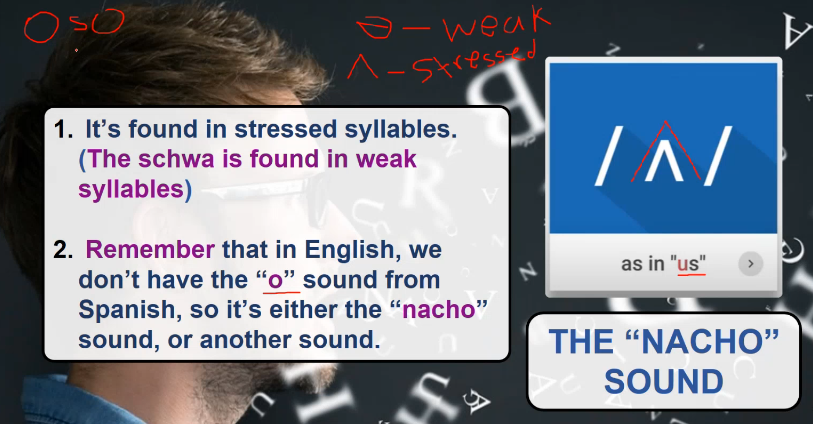
\includegraphics[width=1\textwidth]{images/nacho_portrait.png}
\end{center}

\href{https://drive.google.com/file/d/1YvsXjjdsH54Ibnmu6o0RFniyT1CjNxCH/view?usp=drive_link}{Click here to listen}

\begin{longtable}[c]{||l|l||l|l||}
  \hline
  \textcolor{fancyorange}{Word} & \textcolor{fancyorange}{IPA} & \textcolor{fancyorange}{Word} & \textcolor{fancyorange}{IPA} \\
  \hline
  \textcolor{fancyorange}{U}s        & \textipa{/\textturnv s/}                  & To\textcolor{fancyorange}{u}ch     & \textipa{/'t\textturnv t\textesh/} \\
  C\textcolor{fancyorange}{u}p       & \textipa{/'k\textturnv p/}                & B\textcolor{fancyorange}{u}s       & \textipa{/'b\textturnv s/} \\
  D\textcolor{fancyorange}{u}mb      & \textipa{/'d\textturnv m/}                & An\textcolor{fancyorange}{o}ther   & \textipa{/\textschwa 'n\textturnv\dh\textschwa r/} \\
  M\textcolor{fancyorange}{o}nth     & \textipa{/'m\textturnv n\texttheta/}      & \textcolor{fancyorange}{O}ther     & \textipa{/'\textturnv\dh\textschwa r/} \\
  Bl\textcolor{fancyorange}{oo}d     & \textipa{/'bl\textturnv d/}               & W\textcolor{fancyorange}{o}nderful & \textipa{/'w\textturnv nd\textschwa f\textschwa l/} \\
  Ref\textcolor{fancyorange}{u}nd    & \textipa{/'ri:f\textturnv nd/}            & C\textcolor{fancyorange}{o}me      & \textipa{/'k\textturnv m/} \\
  C\textcolor{fancyorange}{ou}ntry   & \textipa{/'k\textturnv ntri/}             & L\textcolor{fancyorange}{u}ck      & \textipa{/'l\textturnv k/} \\
  C\textcolor{fancyorange}{ou}sin    & \textipa{/'k\textturnv z\textschwa n/}    & C\textcolor{fancyorange}{u}t       & \textipa{/'k\textturnv t/} \\
  C\textcolor{fancyorange}{u}stomer  & \textipa{/'k\textturnv st\textschwa m\textschwa r/} & L\textcolor{fancyorange}{o}ve      & \textipa{/'l\textturnv v/} \\
  M\textcolor{fancyorange}{o}ney     & \textipa{/'m\textturnv ni/}               & Y\textcolor{fancyorange}{ou}ng     & \textipa{/'j\textturnv \ng/} \\
  M\textcolor{fancyorange}{o}ther    & \textipa{/'m\textturnv\dh\textschwa r/}   & En\textcolor{fancyorange}{ou}gh    & \textipa{/I'n\textturnv f/} \\
  S\textcolor{fancyorange}{o}me      & \textipa{/'s\textturnv m/}                & M\textcolor{fancyorange}{u}ch      & \textipa{/'m\textturnv t\textesh/} \\
  F\textcolor{fancyorange}{u}n       & \textipa{/'f\textturnv n/}                & R\textcolor{fancyorange}{u}n       & \textipa{/'r\textturnv n/} \\
  \hline
\end{longtable}


\begin{itemize}
  \item He didn't tell \textbf{\textcolor{fancyorange}{u}s} anything.
  \item Sorry, but I broke \textbf{an\textcolor{fancyorange}{o}ther} \text{cup}.
  \item Honestly, that's a \textbf{d\textcolor{fancyorange}{u}mb} idea.
  \item I don't think we have \textbf{en\textcolor{fancyorange}{ou}gh} \text{money} for the trip.
  \item How \textbf{m\textcolor{fancyorange}{u}ch} \textbf{honey} do you want for your pancakes?
  \item You always \textbf{r\textcolor{fancyorange}{u}n} out of time so you miss the \textbf{b\textcolor{fancyorange}{u}s} every time.
  \item You're too \textbf{y\textcolor{fancyorange}{ou}ng} to go. \text{Though} \textbf{l\textcolor{fancyorange}{u}ck}, \textbf{b\textcolor{fancyorange}{u}ddy}.
  \item Can I get you \textbf{an\textcolor{fancyorange}{o}ther} \text{cup} of coffee?
  \item How many \textbf{c\textcolor{fancyorange}{ou}ntries} have you visited with your cousin?
  \item I'm having so \text{much} \text{fun} here! It's a \textbf{w\textcolor{fancyorange}{o}nderful} place to live.
  \item I can't see \textbf{bl\textcolor{fancyorange}{oo}d}, so don't show me the \textbf{c\textcolor{fancyorange}{u}t} on your finger.
  \item I \textbf{j\textcolor{fancyorange}{u}st} need \textbf{s\textcolor{fancyorange}{o}me} \textbf{m\textcolor{fancyorange}{o}ney} to take \textbf{an\textcolor{fancyorange}{o}ther} \textbf{b\textcolor{fancyorange}{u}s}.
\end{itemize}

\newpage
\section{"Ah" sound \textipa{/A/}}
\begin{center}
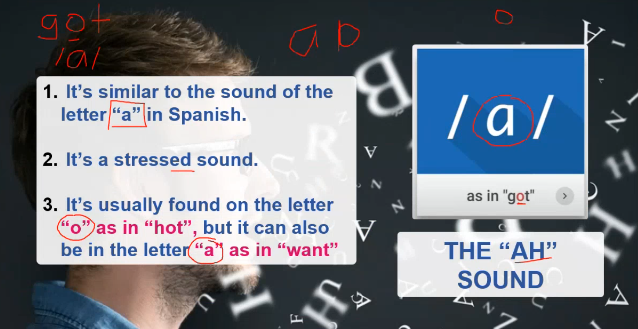
\includegraphics[width=1\textwidth]{images/image5.png}
\end{center}

\href{https://drive.google.com/file/d/18IaOVK4CQk8SdvJZuLdmHg19YmEYxoLD/view?usp=drive_link}{Click here to listen}

\begin{longtable}[c]{||l|l||l|l||}
    \hline
    \textcolor{fancyorange}{Word} & \textcolor{fancyorange}{IPA} & \textcolor{fancyorange}{Word} & \textcolor{fancyorange}{IPA} \\
    \hline
    H\textcolor{fancyorange}{o}t        & \textipa{/h\textscripta t/}             & J\textcolor{fancyorange}{o}b        & \textipa{/d\textyogh\textscripta b/} \\
    C\textcolor{fancyorange}{o}p        & \textipa{/k\textscripta p/}             & \textcolor{fancyorange}{O}pportunity& \textipa{/\textsecstress \textscripta p\textrhookschwa \textprimstress tu\textlengthmark n\textschwa t\textsci/} \\
    G\textcolor{fancyorange}{o}t        & \textipa{/g\textscripta t/}             & J\textcolor{fancyorange}{o}hn       & \textipa{/d\textyogh\textscripta n/} \\
    B\textcolor{fancyorange}{o}ss       & \textipa{/b\textscripta s/}             & N\textcolor{fancyorange}{o}t        & \textipa{/n\textscripta t/} \\
    T\textcolor{fancyorange}{o}p        & \textipa{/t\textscripta p/}             & D\textcolor{fancyorange}{o}cument   & \textipa{/\textprimstress d\textscripta kj\textschwa m\textschwa nt/} \\
    W\textcolor{fancyorange}{a}nt       & \textipa{/w\textscripta nt/}            & D\textcolor{fancyorange}{o}ctor     & \textipa{/\textprimstress d\textscripta kt\textrhookschwa/} \\
    B\textcolor{fancyorange}{o}x        & \textipa{/b\textscripta ks/}            & St\textcolor{fancyorange}{o}p       & \textipa{/st\textscripta p/} \\
    W\textcolor{fancyorange}{a}sh       & \textipa{/w\textscripta \textesh/}      & P\textcolor{fancyorange}{o}ssible   & \textipa{/\textprimstress p\textscripta s\textschwa b\textschwa l/} \\
    B\textcolor{fancyorange}{o}b        & \textipa{/b\textscripta b/}             & Pr\textcolor{fancyorange}{o}blem    & \textipa{/\textprimstress pr\textscripta bl\textschwa m/} \\
    B\textcolor{fancyorange}{o}ttle     & \textipa{/\textprimstress b\textscripta t\textschwa l/} & B\textcolor{fancyorange}{o}dy       & \textipa{/\textprimstress b\textscripta di/} \\
    C\textcolor{fancyorange}{a}lm       & \textipa{/k\textscripta m/}             & L\textcolor{fancyorange}{o}ck       & \textipa{/l\textscripta k/} \\
    C\textcolor{fancyorange}{o}ncert    & \textipa{/\textprimstress k\textscripta ns\textrhookschwa t/} & \textcolor{fancyorange}{O}ption     & \textipa{/\textprimstress \textscripta p\textesh\textschwa n/} \\
    Cl\textcolor{fancyorange}{o}ck      & \textipa{/kl\textscripta k/}            & H\textcolor{fancyorange}{o}nest     & \textipa{/\textprimstress \textscripta n\textschwa st/} \\
    F\textcolor{fancyorange}{o}llow     & \textipa{/\textprimstress f\textscripta lo\textupsilon/} & T\textcolor{fancyorange}{o}pic      & \textipa{/\textprimstress t\textscripta p\textsci k/} \\
    D\textcolor{fancyorange}{o}llar     & \textipa{/\textprimstress d\textscripta l\textrhookschwa/} & Pr\textcolor{fancyorange}{o}duct    & \textipa{/\textprimstress pr\textscripta d\textturnv kt/} \\
    Dr\textcolor{fancyorange}{o}p       & \textipa{/dr\textscripta p/}            & P\textcolor{fancyorange}{o}cket     & \textipa{/\textprimstress p\textscripta k\textschwa t/} \\
    \hline
  \end{longtable}
  
  
  

  
  \begin{itemize}
    \item I don't want to go out it's too \textbf{h\ah{o}t} outside.
    \item \textbf{J\ah{o}hn g\ah{o}t} a new \textbf{j\ah{o}b}, so now he works as a \textbf{c\ah{o}p}.
    \item That's \textbf{n\ah{o}t} a \textbf{pr\ah{o}blem} at all.
    \item \textbf{\ah{O}scar}, can you put the paper in a box and leave it outside?
    \item I just bought an \textbf{\ah{a}partment} and I have all the \textbf{d\ah{o}cuments}.
    \item Should I be in class today? Or should I go to the \textbf{d\ah{o}ctor}?
    \item Can you \textbf{st\ah{o}p} making all that noise?
    \item Is it \textbf{p\ah{o}ssible} to get this done today?
    \item I'm sorry, but that's \textbf{n\ah{o}t} an \textbf{\ah{o}ption}.
    \item Could you \textbf{dr\ah{o}p} Andy at Anna's house?
    \item \textbf{B\ah{o}b} is the new \textbf{b\ah{o}ss} and he has a lot of \textbf{pr\ah{o}blems} to fix at the \textbf{\ah{o}ffice}.
    \item The customer says he got an incorrect \textbf{pr\ah{o}duct}. What should I do?
    \item I'm not awake enough to pay attention to this \textbf{t\ah{o}pic} today.
    \item I'm going to be \textbf{h\ah{o}nest}; I took a few \textbf{d\ah{o}llars} you had in your \textbf{p\ah{o}cket}.
    \item Make sure you \textbf{f\ah{o}llow} the \textbf{pr\ah{o}cess} correctly this time.
  \end{itemize}

  \newpage
\section{"Pretzel" sound \textipa/{\ae}/}
\begin{center}
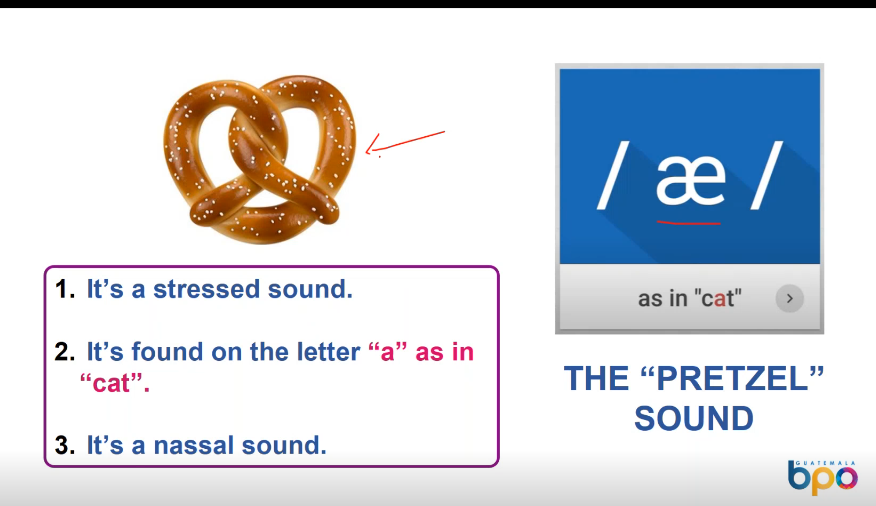
\includegraphics[width=1\textwidth]{images/pretzel_portrait.png}
\end{center}

\href{https://drive.google.com/file/d/1hJGOQVApbcAGU1vvELpt-nEejQ8-av7o/view?usp=drive_link}{Click here to listen}

\begin{longtable}[c]{||l|l||l|l||}
  \hline
  \textcolor{fancyorange}{Word} & \textcolor{fancyorange}{IPA} & \textcolor{fancyorange}{Word} & \textcolor{fancyorange}{IPA} \\
  \hline
  C\textcolor{fancyorange}{a}t     & \textipa{/'k\ae t/}                         & C\textcolor{fancyorange}{a}p       & \textipa{/'k\ae p/} \\
  H\textcolor{fancyorange}{a}t     & \textipa{/'h\ae t/}                         & F\textcolor{fancyorange}{a}st      & \textipa{/'f\ae st/} \\
  M\textcolor{fancyorange}{a}n     & \textipa{/'m\ae n/}                         & E\textcolor{fancyorange}{x}ample   & \textipa{/\textsci g'z\ae mp\textschwa l/} \\
  A\textcolor{fancyorange}{d}d     & \textipa{/'\ae d/}                          & \textcolor{fancyorange}{A}ccident  & \textipa{/'\ae ks\textschwa d\textschwa nt/} \\
  M\textcolor{fancyorange}{a}nager & \textipa{/'m\ae n\textschwa d\textyogh\textschwa r/} & S\textcolor{fancyorange}{a}turday  & \textipa{/'s\ae t\textsubarch\textrhookschwa . d\textsci/} \\
  \textcolor{fancyorange}{A}pple   & \textipa{/'\ae p\textschwa l/}             & F\textcolor{fancyorange}{a}mily    & \textipa{/'f\ae m\textschwa li/} \\
  \textcolor{fancyorange}{A}sk     & \textipa{/'\ae sk/}                         & Cl\textcolor{fancyorange}{a}ss     & \textipa{/'kl\ae s/} \\
  B\textcolor{fancyorange}{a}ck    & \textipa{/'b\ae k/}                         & L\textcolor{fancyorange}{a}st      & \textipa{/'l\ae st/} \\
  B\textcolor{fancyorange}{a}d     & \textipa{/'b\ae d/}                         & H\textcolor{fancyorange}{a}bit     & \textipa{/'h\ae b\textsci t/} \\
  S\textcolor{fancyorange}{a}d     & \textipa{/'s\ae d/}                         & \textcolor{fancyorange}{A}nswer    & \textipa{/'\ae n\textschwa r/} \\
  J\textcolor{fancyorange}{a}cket  & \textipa{/'d\textyogh\ae k\textschwa t/}    & \textcolor{fancyorange}{A}nimal    & \textipa{/'\ae n\textschwa m\textschwa l/} \\
  P\textcolor{fancyorange}{a}st    & \textipa{/'p\ae st/}                        & C\textcolor{fancyorange}{a}tch     & \textipa{/'k\ae t\textesh/} \\
  \hline
\end{longtable}
  
\begin{itemize}
  \item \textbf{Th\textcolor{fancyorange}{a}t} \textbf{m\textcolor{fancyorange}{a}n} loves putting \textbf{h\textcolor{fancyorange}{a}ts} on his \textbf{f\textcolor{fancyorange}{a}t} \textbf{c\textcolor{fancyorange}{a}t}.
  \item There was an \textbf{\textcolor{fancyorange}{a}ccident} on my way \textbf{b\textcolor{fancyorange}{a}ck} from work.
  \item I \textbf{h\textcolor{fancyorange}{a}ve} an important test on \textbf{S\textcolor{fancyorange}{a}turday}, so I \textbf{c\textcolor{fancyorange}{a}n't} \textbf{h\textcolor{fancyorange}{a}ng} out with you.
  \item Is \textbf{th\textcolor{fancyorange}{a}t} an \textbf{\textcolor{fancyorange}{a}pple} pie? I'm starving, and it smells delicious.
  \item Why are you eating like an \textbf{\textcolor{fancyorange}{a}nimal}? Slow down a little bit.
  \item The \textbf{l\textcolor{fancyorange}{a}st} time I gave you my \textbf{j\textcolor{fancyorange}{a}cket}, you lost it.
  \item My \textbf{f\textcolor{fancyorange}{a}mily} is going to \textbf{g\textcolor{fancyorange}{a}ther} around and \textbf{c\textcolor{fancyorange}{a}tch} up on \textbf{S\textcolor{fancyorange}{a}turday}.
  \item I don't want to talk to another \textbf{m\textcolor{fancyorange}{a}nager}. I just need an \textbf{\textcolor{fancyorange}{a}nswer}.
  \item \textbf{Th\textcolor{fancyorange}{a}t} \textbf{m\textcolor{fancyorange}{a}n} told me a story, but it doesn't \textbf{\textcolor{fancyorange}{a}dd} up.
  \item Eating when you're \textbf{s\textcolor{fancyorange}{a}d} and bored isn't a good idea.
  \item I \textbf{h\textcolor{fancyorange}{a}d} an \textbf{\textcolor{fancyorange}{a}ccident} \textbf{l\textcolor{fancyorange}{a}st} week.
  \item I'll be \textbf{b\textcolor{fancyorange}{a}ck} as soon as I \textbf{c\textcolor{fancyorange}{a}n}.
  \item If you need an \textbf{ex\textcolor{fancyorange}{a}mple}, google it.
  \item The cop got all the \textbf{\textcolor{fancyorange}{a}nswers} without \textbf{\textcolor{fancyorange}{a}sking} anything.
\end{itemize}

\newpage
\section{"EH" sound as in "bet" \textipa{/e/}}
\begin{center}
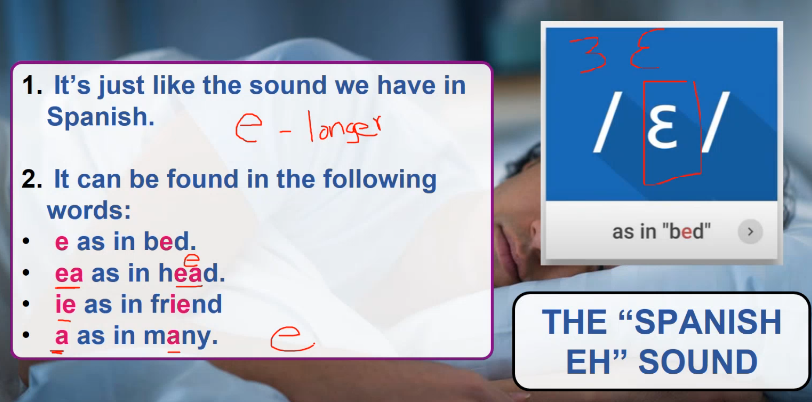
\includegraphics[width=1\textwidth]{images/eh_portrait.png}
\end{center}

\href{https://drive.google.com/file/d/1OyxdLbyCPaULwdQg9UnMv6D7VTytreMO/view?usp=drive_link}{Click here to listen}

% \begin{longtable}[c]{||l|l||}
%   \hline
%   \textcolor{fancyorange}{Word} & \textcolor{fancyorange}{IPA} \\
%   \hline
%   % Bed
%   B\textcolor{fancyorange}{e}d      & \textipa{/b\textepsilon d/} \\
%   % Get
%   G\textcolor{fancyorange}{e}t      & \textipa{/g\textepsilon t/} \\
%   \hline
%   % Head
%   H\textcolor{fancyorange}{e}ad    & \textipa{/h\textepsilon d/} \\
%   % Friend
%   Fr\textcolor{fancyorange}{e}nd   & \textipa{/fr\textepsilon n d/} \\
%   % Again
%   Ag\textcolor{fancyorange}{a}in   & \textipa{/\textschwa'g\textepsilon n/} \\
%   % Met
%   M\textcolor{fancyorange}{e}t      & \textipa{/m\textepsilon t/} \\
%   % Said
%   S\textcolor{fancyorange}{a}id    & \textipa{/s\textepsilon d/} \\
%   % Says
%   S\textcolor{fancyorange}{a}ys    & \textipa{/s\textepsilon z/} \\
%   % Let
%   L\textcolor{fancyorange}{e}t      & \textipa{/l\textepsilon t/} \\
%   % Sell
%   S\textcolor{fancyorange}{e}ll    & \textipa{/s\textepsilon l/} \\
%   % Tell
%   T\textcolor{fancyorange}{e}ll    & \textipa{/t\textepsilon l/} \\
%   % Fell
%   F\textcolor{fancyorange}{e}ll    & \textipa{/f\textepsilon l/} \\
%   % Well
%   W\textcolor{fancyorange}{e}ll    & \textipa{/w\textepsilon l/} \\
%   % Yell
%   Y\textcolor{fancyorange}{e}ll    & \textipa{/j\textepsilon l/} \\
%   % Men
%   M\textcolor{fancyorange}{e}n      & \textipa{/m\textepsilon n/} \\
%   % Debt
%   D\textcolor{fancyorange}{e}bt    & \textipa{/d\textepsilon t/} \\
%   % Yet
%   Y\textcolor{fancyorange}{e}t      & \textipa{/j\textepsilon t/} \\
%   % Mention
%   M\textcolor{fancyorange}{e}ntion & \textipa{/\textprimstress m\textepsilon n\textesh\textschwa n/} \\
%   % Second
%   S\textcolor{fancyorange}{e}cond  & \textipa{/\textprimstress s\textepsilon k\textrhookschwa n/} \\
%   % Credit
%   Cr\textcolor{fancyorange}{e}dit  & \textipa{/'kr\textepsilon d\textsci t/} \\
%   % Seven
%   S\textcolor{fancyorange}{e}ven  & \textipa{/\textprimstress s\textepsilon v\textepsilon n/} \\
%   % Sweater
%   Sw\textcolor{fancyorange}{e}ater & \textipa{/\textprimstress sw\textepsilon t\textschwa r/} \\
%   % Swear
%   Sw\textcolor{fancyorange}{e}ar   & \textipa{/\textprimstress sw\textepsilon r/} \\
%   % Celebrity
%   C\textcolor{fancyorange}{e}lebrity & \textipa{/\textprimstress s\textepsilon l\textschwa b\textschwa r\textepsilon t\textrhookschwa/} \\
%   % Bread
%   Br\textcolor{fancyorange}{e}ad   & \textipa{/\textprimstress b\textepsilon d/} \\
%   % Breath
%   Br\textcolor{fancyorange}{e}ath & \textipa{/\textprimstress b\textepsilon \textesh/} \\
%   \hline  
% \end{longtable}

\begin{longtable}[c]{||l|l||l|l||}
  \hline
  \textcolor{fancyorange}{Word} & \textcolor{fancyorange}{IPA} & \textcolor{fancyorange}{Word} & \textcolor{fancyorange}{IPA} \\
  \hline
  B\textcolor{fancyorange}{e}d      & \textipa{/b\textepsilon d/}               & Y\textcolor{fancyorange}{e}ll      & \textipa{/j\textepsilon l/}             \\
  G\textcolor{fancyorange}{e}t      & \textipa{/g\textepsilon t/}               & M\textcolor{fancyorange}{e}n       & \textipa{/m\textepsilon n/}             \\
  H\textcolor{fancyorange}{e}ad     & \textipa{/h\textepsilon d/}               & D\textcolor{fancyorange}{e}bt      & \textipa{/d\textepsilon t/}             \\
  Fri\textcolor{fancyorange}{e}nd   & \textipa{/fr\textepsilon nd/}             & Y\textcolor{fancyorange}{e}t       & \textipa{/j\textepsilon t/}             \\
  Ag\textcolor{fancyorange}{ai}n    & \textipa{/\textschwa'g\textepsilon n/}    & M\textcolor{fancyorange}{e}ntion   & \textipa{/\textprimstress m\textepsilon n\textesh\textschwa n/} \\
  M\textcolor{fancyorange}{e}t      & \textipa{/m\textepsilon t/}               & S\textcolor{fancyorange}{e}cond    & \textipa{/\textprimstress s\textepsilon k\textrhookschwa n/}     \\
  S\textcolor{fancyorange}{ai}d     & \textipa{/s\textepsilon d/}               & Cr\textcolor{fancyorange}{e}dit    & \textipa{/'kr\textepsilon d\textsci t/}                         \\
  S\textcolor{fancyorange}{a}ys     & \textipa{/s\textepsilon z/}               & S\textcolor{fancyorange}{e}ven     & \textipa{/\textprimstress s\textepsilon v\textepsilon n/}       \\
  L\textcolor{fancyorange}{e}t      & \textipa{/l\textepsilon t/}               & Sw\textcolor{fancyorange}{e}ater   & \textipa{/\textprimstress sw\textepsilon t\textschwa r/}        \\
  S\textcolor{fancyorange}{e}ll     & \textipa{/s\textepsilon l/}               & Sw\textcolor{fancyorange}{ea}r     & \textipa{/\textprimstress sw\textepsilon r/}                    \\
  T\textcolor{fancyorange}{e}ll     & \textipa{/t\textepsilon l/}               & C\textcolor{fancyorange}{e}lebrity & \textipa{/\textprimstress s\textepsilon l\textschwa b\textschwa r\textepsilon t\textrhookschwa/} \\
  F\textcolor{fancyorange}{e}ll     & \textipa{/f\textepsilon l/}               & Br\textcolor{fancyorange}{e}ad     & \textipa{/\textprimstress br\textepsilon d/}                     \\
  W\textcolor{fancyorange}{e}ll     & \textipa{/w\textepsilon l/}               & Br\textcolor{fancyorange}{e}ath    & \textipa{/\textprimstress br\textepsilon \texttheta/}             \\
  \hline
\end{longtable}



\begin{itemize}
  \item[A:] So, what time did you \textbf{go to b\textcolor{fancyorange}{e}d} last night?
  \item[B:] I \textbf{w\textcolor{fancyorange}{e}nt to b\textcolor{fancyorange}{e}d} at 1 am because I was playing videogames. And you? What time do you usually go to \textbf{b\textcolor{fancyorange}{e}d}?
\end{itemize}

\begin{itemize}
  \item[A:] My brother got into a lot of \textbf{d\textcolor{fancyorange}{e}bts} because he loves using his \textbf{cr\textcolor{fancyorange}{e}dit} card.
  \item[B:] Yeah, doing that isn't a good idea. Do you think it's necessary to \textbf{g\textcolor{fancyorange}{e}t} into \textbf{d\textcolor{fancyorange}{e}bts} by using a \textbf{cr\textcolor{fancyorange}{e}dit} card?
\end{itemize}

\begin{itemize}
  \item[A:] Teams is suck again! I think I'm going to lose my \textbf{h\textcolor{fancyorange}{e}ad} today.
  \item[B:] I know that Teams is annoying, but don't lose your \textbf{h\textcolor{fancyorange}{e}ad}. Just take a deep \textbf{br\textcolor{fancyorange}{e}ath}. What other things make you lose your \textbf{h\textcolor{fancyorange}{e}ad} sometimes?
\end{itemize}

\begin{itemize}
  \item[A:] Sorry, I didn't hear anything you \textbf{s\textcolor{fancyorange}{a}id}. What are we supposed to do?
  \item[B:] You always have your \textbf{h\textcolor{fancyorange}{e}ad} in the clouds when you're in class. Why are you so distracted?
\end{itemize}

\begin{itemize}
  \item[A:] I like my new job, and I'm making a lot of \textbf{fr\textcolor{fancyorange}{ie}nds} already.
  \item[B:] Really? I'm not good at making \textbf{fr\textcolor{fancyorange}{ie}nds} with people. Any suggestions?
\end{itemize}

\begin{itemize}
  \item[A:] I \textbf{m\textcolor{fancyorange}{e}t} up with an old friend last week. He \textbf{s\textcolor{fancyorange}{a}id} he's been traveling a lot.
  \item[B:] Oh, I see. Personally, I don't think I would enjoy \textbf{trav\textcolor{fancyorange}{e}lling} so often. And you?
\end{itemize}

\begin{itemize}
  \item[A:] Can you give me a \textbf{s\textcolor{fancyorange}{e}cond}? I need to restart my router again.
  \item[B:] No problem. \textbf{L\textcolor{fancyorange}{e}t} me know \textbf{wh\textcolor{fancyorange}{e}n} you're back.
\end{itemize}

\begin{itemize}
  \item[A:] Are you ok? You're out of \textbf{br\textcolor{fancyorange}{e}ath}.
  \item[B:] Yeah, I had to take the \textbf{st\textcolor{fancyorange}{e}ps}. I \textbf{gu\textcolor{fancyorange}{e}ss} I need to do more exercise. How often do you exercise?
\end{itemize}

\begin{itemize}
  \item[A:] \textbf{B\textcolor{fancyorange}{e}n} \textbf{s\textcolor{fancyorange}{a}ys} he \textbf{f\textcolor{fancyorange}{e}ll} in love with a girl last month and that he's going to marry her.
  \item[B:] He always \textbf{s\textcolor{fancyorange}{a}ys} that. I \textbf{b\textcolor{fancyorange}{e}t} she's going to break up with him in a few weeks.
\end{itemize}

\begin{itemize}
  \item[A:] I hate this \textbf{w\textcolor{fancyorange}{e}ather}. I \textbf{sw\textcolor{fancyorange}{e}at} all the time and I'm always thirsty.
  \item[B:] Oh I know. I feel like taking a shower \textbf{ag\textcolor{fancyorange}{a}in} and \textbf{ag\textcolor{fancyorange}{a}in} when the day is hot.
\end{itemize}

\begin{itemize}
  \item[A:] Can you \textbf{l\textcolor{fancyorange}{e}nd} me Q1,000? I swear I'm going to pay you in a few days.
  \item[B:] \textbf{Ag\textcolor{fancyorange}{a}in}? Why do you always \textbf{g\textcolor{fancyorange}{e}t} into \textbf{d\textcolor{fancyorange}{e}bts}? Sorry, but I can't \textbf{l\textcolor{fancyorange}{e}nd} you any more money.
\end{itemize}

\begin{itemize}
  \item[A:] I need to \textbf{g\textcolor{fancyorange}{e}t} \textbf{b\textcolor{fancyorange}{e}tter} at remembering vocabulary. I'm lost.
  \item[B:] Yeah I know, but it takes time and practice. \textbf{W\textcolor{fancyorange}{e}'re} doing fine.
\end{itemize}

\newpage







\section{"AW" sound as in "thought" \textipa{/\textopeno/}}
\begin{center}
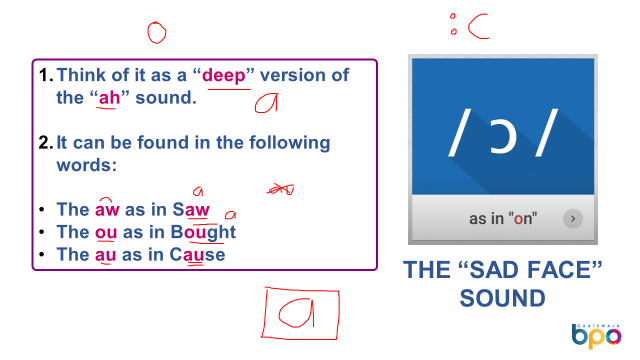
\includegraphics[width=1\textwidth]{images/sad_face_portrait.png}
\end{center}

\href{https://drive.google.com/file/d/154q9gt0WLnpRNkAjcv0uexXSiC0pnEYK/view?usp=drive_link}{Click here to listen}

\begin{longtable}[c]{||l|l||l|l||}
  \hline
  \textcolor{fancyorange}{Word} & \textcolor{fancyorange}{IPA} & \textcolor{fancyorange}{Word} & \textcolor{fancyorange}{IPA} \\
  \hline
  \textbf{B\textcolor{fancyorange}{ough}t}     & \textipa{'b\textopeno t} & \textbf{F\textcolor{fancyorange}{au}lt}      & \textipa{'f\textopeno lt} \\
  \textbf{Dr\textcolor{fancyorange}{aw}}       & \textipa{'d\textturnr\textopeno} & \textbf{F\textcolor{fancyorange}{ough}t}     & \textipa{'f\textopeno t} \\
  \textbf{S\textcolor{fancyorange}{aw}}        & \textipa{'s\textopeno} & \textbf{D\textcolor{fancyorange}{augh}ter}   & \textipa{'d\textopeno\textturnt\textschwa\textturnr} \\
  \textbf{Br\textcolor{fancyorange}{ough}t}    & \textipa{'b\textturnr\textopeno t} & \textbf{L\textcolor{fancyorange}{aw}yer}     & \textipa{'l\textopeno.\textschwa\textturnr} \\
  \textbf{C\textcolor{fancyorange}{a}ll}       & \textipa{'k\textopeno l} & \textbf{L\textcolor{fancyorange}{aw}}        & \textipa{'l\textopeno} \\
  \textbf{C\textcolor{fancyorange}{augh}t}     & \textipa{'k\textopeno t} & \textbf{\textcolor{fancyorange}{Au}gust}     & \textipa{,\textopeno'g\textschwa st} \\
  \textbf{T\textcolor{fancyorange}{augh}t}     & \textipa{'t\textopeno t} & \textbf{\textcolor{fancyorange}{Au}thor}     & \textipa{'\textopeno\texttheta\textschwa\textturnr} \\
  \textbf{Th\textcolor{fancyorange}{ough}t}    & \textipa{'\texttheta\textopeno t} & \textbf{T\textcolor{fancyorange}{a}lk}       & \textipa{'t\textopeno k} \\
  \textbf{C\textcolor{fancyorange}{au}se}      & \textipa{'k\textopeno z} & \textbf{W\textcolor{fancyorange}{a}lk}       & \textipa{'w\textopeno k} \\
  \textbf{C\textcolor{fancyorange}{ough}}      & \textipa{'k\textopeno f} & \textbf{\textcolor{fancyorange}{Aw}esome}    & \textipa{'\textopeno s\textschwa m} \\
  \textbf{D\textcolor{fancyorange}{aw}n}       & \textipa{'d\textopeno n} & \textbf{\textcolor{fancyorange}{Au}dio}      & \textipa{'\textopeno.di.o\textupsilon} \\
  \textbf{D\textcolor{fancyorange}{o}g}        & \textipa{'d\textopeno g} & \textbf{\textcolor{fancyorange}{Aw}ful}      & \textipa{'\textopeno f\textschwa l} \\
  \textbf{F\textcolor{fancyorange}{a}ll}       & \textipa{'f\textopeno l} & \textbf{Fr\textcolor{fancyorange}{au}d}      & \textipa{'f\textturnr\textopeno d} \\
  \hline
\end{longtable}

\begin{itemize}
  \item[A] Why did you buy a new phone? Don't you have one already?
  \item[B] Well, I \textbf{bought} a new phone because I'm going to give it to my mom. She said she wanted to learn how to use one.
\end{itemize}

\begin{itemize}
  \item[A] I didn't know you could \textbf{draw}. These are amazing!
  \item[B] Thanks! I've been practicing for months now, and I want to become a professional artist.  
\end{itemize}

\begin{itemize}
  \item[A] I \textbf{saw} you yesterday and I waved my hand, but you didn't say hi. Why did you ignore me?
  \item[B] Oh I \textbf{thought} you were someone else. Sorry, but didn't have my glasses, so I didn't recognize you. 
\end{itemize}

\begin{itemize}
  \item[A] I'm sorry for forgetting your birthday last month, but I \textbf{brought} you some pizza!
  \item[B] I'm still angry with you, but since I love pizza I will forgive you for now. 
\end{itemize}

\begin{itemize}
  \item[A] So George, who's your favorite \textbf{author}?
  \item[B] Honestly, reading isn't my cup of tea, so I really don't know any \textbf{authors}. 
\end{itemize}

\begin{itemize}
  \item[A] George \textbf{caught} me sleeping in class, and I couldn't come up with an excuse.
  \item[B] I \textbf{thought} you were going to start going to bed earlier in order to have more energy for the class. What happened? 
\end{itemize}

\begin{itemize}
  \item[A] Did you really play videogames until \textbf{dawn}? How are you going to be awake for the class ?
  \item[B] Relax, George, I just need a RedBull, a Raptor and a coffee, and I'll be just fine.  
\end{itemize}

\begin{itemize}
  \item[A] I paid \$1,000.00 for the Iphone 16 on Facebook Marketplace, but now the vendor isn't answering my messages.
  \item[B] How could you \textbf{fall} for that? It was clearly a scam. Sorry, but that money is now gone. 
\end{itemize}

\begin{itemize}
  \item[A] Did you hear about John? He got \textbf{caught} red-handed stealing money from customers.
  \item[B] Really? I never \textbf{thought} he would break the \textbf{law}. What's going to happen to him now ?  
\end{itemize}

\begin{itemize}
  \item[A] So, how did the date go?
  \item[B] Oh it was \textbf{awful}! I was stood up, so I didn't even meet the person.  
\end{itemize}

\begin{itemize}
  \item[A] Well, I \text{thought} the movie was going to be \textbf{awesome}, but it was disappointing.
  \item[B] I \textbf{saw} it last week and I \textbf{thought} it was just OK. 
\end{itemize}

\begin{itemize}
  \item[A] Why are you mad at me? It wasn't my \textbf{fault} that you got an F on your test.
  \item[B] Of \textbf{course} it was your \textbf{fault}! You knew we would have a surprise test and you didn't tell me. 
\end{itemize}

\newpage







\section{"UH" sound as in "book" \textipa{/ \textupsilon /}}
\begin{center}
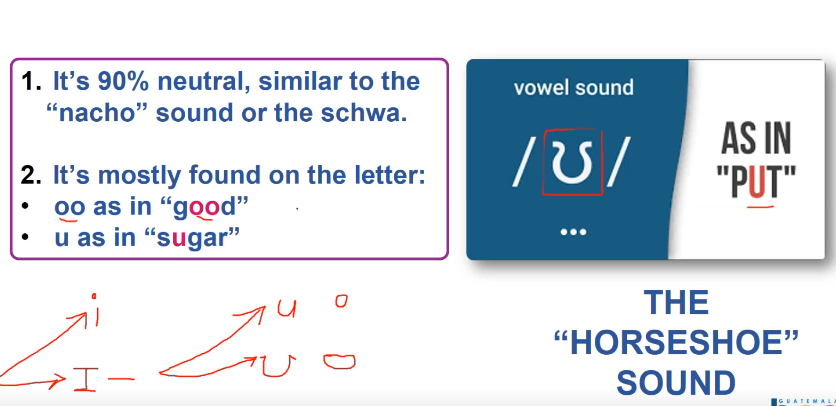
\includegraphics[width=1\textwidth]{images/horseshoe_portrait.png}
\end{center}

\href{https://drive.google.com/file/d/1tOw8dRxqQy4Pn4bsapMfJOim9e4x7oKU/view?usp=sharing}{Click here to listen}

\begin{longtable}[c]{||l|l||l|l||}
  \hline
  \textcolor{fancyorange}{Word} & \textcolor{fancyorange}{IPA} & \textcolor{fancyorange}{Word} & \textcolor{fancyorange}{IPA} \\
  \hline
  \textbf{F\textcolor{fancyorange}{u}ll} & \textipa{/'f\textupsilon l/} & \textbf{Sh\textcolor{fancyorange}{ou}ld} & \textipa{/'\textesh\textupsilon d/} \\
  \textbf{P\textcolor{fancyorange}{u}t} & \textipa{/'p\textupsilon t/} & \textbf{W\textcolor{fancyorange}{ou}ld} & \textipa{/'w\textupsilon d/} \\
  \textbf{P\textcolor{fancyorange}{u}ll} & \textipa{/'p\textupsilon l/} & \textbf{C\textcolor{fancyorange}{oo}kie} & \textipa{/'k\textupsilon ki/} \\
  \textbf{S\textcolor{fancyorange}{u}gar} & \textipa{/'\textesh\textupsilon g\textschwa\textturnr/} & \textbf{T\textcolor{fancyorange}{oo}k} & \textipa{/'t\textupsilon k/} \\
  \textbf{B\textcolor{fancyorange}{oo}k} & \textipa{/'b\textupsilon k/} & \textbf{P\textcolor{fancyorange}{u}sh} & \textipa{/'p\textupsilon \textesh/} \\
  \textbf{C\textcolor{fancyorange}{oo}k} & \textipa{/'k\textupsilon k/} & \textbf{W\textcolor{fancyorange}{o}man} & \textipa{/'w\textupsilon m\textschwa n/} \\
  \textbf{F\textcolor{fancyorange}{oo}t} & \textipa{/'f\textupsilon t/} & \textbf{Childh\textcolor{fancyorange}{oo}d} & \textipa{/'t\textesh a\textsci ld.h\textupsilon d/} \\
  \textbf{G\textcolor{fancyorange}{oo}d} & \textipa{/'g\textupsilon d/} & \textbf{C\textcolor{fancyorange}{u}shion} & \textipa{/'k\textupsilon \textesh\textschwa n/} \\
  \textbf{L\textcolor{fancyorange}{oo}k} & \textipa{/'l\textupsilon k/} & \textbf{B\textcolor{fancyorange}{u}lly} & \textipa{/'b\textupsilon li/} \\
  \textbf{C\textcolor{fancyorange}{ou}ld} & \textipa{/'k\textupsilon d/} & \textbf{H\textcolor{fancyorange}{oo}die} & \textipa{/'h\textupsilon di/} \\
  \hline  
\end{longtable}

\begin{itemize}
  \item You \textbf{took} my \textbf{hoodie}, didn't you? Why do yo always take my clothes?
  \item I think I have a problem with \textbf{sugar}, I can't stop eating sweet things. Do you have the same problem?
  \item What's a \textbf{childhood} memory that you cherish? For example, I used to visit my grandma a lot when I was a child.
  \item In your opinion, what's a thing we \textbf{should} do more often to improve our fluency?
  \item What kind of shift are you looking for right now? An AM shift or a PM shift?
  \item I'm not \textbf{good} at using Excel, although I think I \textbf{should} learn to use it. What about you?
  \item Do you like \textbf{books} or movies? If, so, what kind of movies or \textbf{books} are you into?
  \item What's a thing that \textbf{puts} you in a \textbf{good} mood? A song, a snack, a show?
  \item Is it true that we're going to leave early today or are you just \textbf{pulling my leg}?
  \item \textbf{Would} you like to go to the movies tonight? I have two tickets.
  \item I hurt my \textbf{foot} while I was walking and now it's swollen. What do you recommend?
  \item My cousin is so \textbf{full} of himself. He's always talking about his achievements and how great he is. Do you know anyone like that?
\end{itemize}


\newpage







\section{"Long U" sound as in "usually" \textipa{/ju/}}
\begin{center}
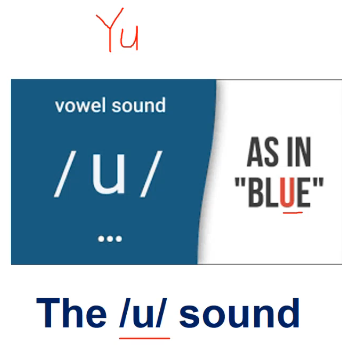
\includegraphics[width=1\textwidth]{images/long_u_portrait.png}
\end{center}

\href{https://drive.google.com/file/d/1d3kXrZ-ctq1nlfgTstKuc3zmRYpuEt42/view?usp=sharing}{Click here to listen}

\begin{longtable}[c]{||l|l||l|l||}
  \hline
  \textcolor{fancyorange}{Word} & \textcolor{fancyorange}{IPA} &
  \textcolor{fancyorange}{Word} & \textcolor{fancyorange}{IPA} \\
  \hline
  \textbf{M\textcolor{fancyorange}{oo}n}       & \textipa{/'mu\textlengthmark n/} &
  \textbf{So\textcolor{fancyorange}{u}p}       & \textipa{/'su\textlengthmark p/} \\
  \textbf{Ch\textcolor{fancyorange}{oo}se}     & \textipa{/'t\textesh u\textlengthmark z/} &
  \textbf{M\textcolor{fancyorange}{o}ve}       & \textipa{/'mu\textlengthmark v/} \\
  \textbf{C\textcolor{fancyorange}{oo}l}       & \textipa{/'ku\textlengthmark l/} &
  \textbf{Wh\textcolor{fancyorange}{o}}        & \textipa{/'hu\textlengthmark /} \\
  \textbf{F\textcolor{fancyorange}{oo}l}       & \textipa{/'fu\textlengthmark l/} &
  \textbf{M\textcolor{fancyorange}{oo}d}       & \textipa{/'mu\textlengthmark d/} \\
  \textbf{P\textcolor{fancyorange}{oo}l}       & \textipa{/'pu\textlengthmark l/} &
  \textbf{Y\textcolor{fancyorange}{ou}}        & \textipa{/'ju\textlengthmark /} \\
  \textbf{L\textcolor{fancyorange}{oo}se}      & \textipa{/'lu\textlengthmark s/} &
  \textbf{Comp\textcolor{fancyorange}{u}ter}   & \textipa{/,k\textschwa m'pju\textlengthmark \textturnr /} \\
  \textbf{L\textcolor{fancyorange}{o}se}       & \textipa{/'lu\textlengthmark z/} &
  \textbf{Dis\textcolor{fancyorange}{pu}te}    & \textipa{/,d\textsci'spju\textlengthmark t/} \\
  \textbf{Sch\textcolor{fancyorange}{oo}l}     & \textipa{/'sku\textlengthmark l/} &
  \textbf{\textcolor{fancyorange}{U}sually}    & \textipa{/'ju\textlengthmark \textyogh \textschwa l\textsci/} \\
  \textbf{S\textcolor{fancyorange}{oo}n}       & \textipa{/'su\textlengthmark n/} &
  \textbf{Amb\textcolor{fancyorange}{u}lance}  & \textipa{/'{\ae}mbj\textschwa l\textschwa ns/} \\
  \textbf{R\textcolor{fancyorange}{u}le}       & \textipa{/'\textturnr u\textlengthmark l/} &
  \textbf{M\textcolor{fancyorange}{u}te}       & \textipa{/'mju\textlengthmark t/} \\
  \textbf{Fl\textcolor{fancyorange}{u}}        & \textipa{/'flu\textlengthmark /} &
  \textbf{Sing\textcolor{fancyorange}{u}lar}   & \textipa{/'s\textsci\ng gj\textschwa l\textturnr /} \\
  \textbf{Bl\textcolor{fancyorange}{ew}}       & \textipa{/'blu\textlengthmark /} &
  \textbf{Partic\textcolor{fancyorange}{u}lar} & \textipa{/'p\textschwa t\textsci kj\textschwa l\textturnr /} \\
  \textbf{Ch\textcolor{fancyorange}{ew}}       & \textipa{/'t\textesh u\textlengthmark /} &
  \textbf{\textcolor{fancyorange}{U}se (noun)} & \textipa{/'ju\textlengthmark s/} \\
  \textbf{Gr\textcolor{fancyorange}{ou}p}      & \textipa{/'g\textturnr u\textlengthmark p/} &
  \textbf{Doc\textcolor{fancyorange}{u}ment}   & \textipa{/'d\textopeno kj\textschwa m\textschwa nt/} \\
  \hline
\end{longtable}

\begin{itemize}
  \item So, George, why were you so \textbf{over the moon} yesterday? What happened?
  \item Alright, so if you were me, what would you \textbf{choose}? Working in the morning or working in the afternoon? Why?
  \item George, would you describe yourself as a \textbf{cool-headed} person or as hot-headed person? \textbf{(Someone that's usually calm even in difficult situations)}
  \item I saw you \textbf{fooling around} instead of working in class this morning. Why didn't you want to work? \textbf{(To waste time instead of working or being productive)}
  \item This traffic is not moving \textbf{anytime soon}, so let's \textbf{hang loose} and listen to some \textbf{music}. What would you like to listen to? \textbf{(When you hang loose, you wait patiently)}
  \item I have a friend that couldn't pass his first job interview, and I don't want him to \textbf{lose heart}. What do you think I can tell him? \textbf{(To feel discouraged and stop believing you can succeed)}
  \item You know, \textbf{as soon as} the class is over I take a nap. How about you?
  \item I went on a date last Saturday and by mistake I called my date by the wrong name and then I spilled my drink all over the table. Do you think I \textbf{blew it}? \textbf{(To make a big mistake or ruin a moment or opportunity)}
  \item George, I think I'm in a \textbf{bad mood} today, but what can I do to get in a \textbf{better mood}?
  \item Is it \textbf{usual} for you to stay up on weekdays? What about the weekends?
  \item George says he won't let us go early anymore. Should we keep asking or \textbf{there's no use talking} to him? \textbf{(When doing something is pointless or useless)}
  \item So, George, do you have a \textbf{particular} method for practicing English alone or do you just practice in class?
\end{itemize}




\newpage







\section{"ER" sound as in "girl", "first", "bird" \textipa{/\textschwa\textturnr}/}
\begin{center}
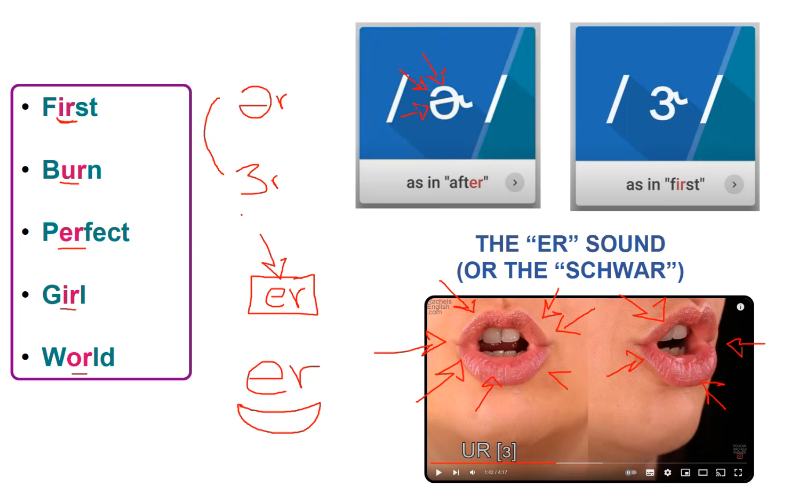
\includegraphics[width=1\textwidth]{images/er_portrait.png}
\end{center}

\href{https://drive.google.com/file/d/1c1VYP8y_y8aZ3aMOANftbIooVzKmxFav/view?usp=sharing}{Click here to listen}

\begin{longtable}[c]{||l|l||l|l||}
  \hline
  \textcolor{fancyorange}{Word} & \textcolor{fancyorange}{IPA} &
  \textcolor{fancyorange}{Word} & \textcolor{fancyorange}{IPA} \\
  \hline
  \textbf{First} & \textipa{/'f\textschwa\textturnr st/} & \textbf{G\textcolor{fancyorange}{ir}l} & \textipa{/'g\textschwa\textturnr l/} \\
  \textbf{Ans\textcolor{fancyorange}{wer}} & \textipa{/'{\ae}n.s\textschwa\textturnr/} & \textbf{W\textcolor{fancyorange}{or}d} & \textipa{/'w\textschwa\textturnr d/} \\
  \textbf{B\textcolor{fancyorange}{ir}d} & \textipa{/'b\textschwa\textturnr d/} & \textbf{W\textcolor{fancyorange}{or}ld} & \textipa{/'w\textschwa\textturnr ld/} \\
  \textbf{B\textcolor{fancyorange}{ir}thday} & \textipa{/'b\textschwa\textturnr\texttheta.de\textsci/} & \textbf{W\textcolor{fancyorange}{or}k} & \textipa{/'w\textschwa\textturnr k/} \\
  \textbf{Decemb\textcolor{fancyorange}{er}} & \textipa{/d\textsci's\textepsilon m.b\textschwa\textturnr/} & \textbf{D\textcolor{fancyorange}{ir}ty} & \textipa{/'d\textschwa\textturnr.ti/} \\
  \textbf{Bett\textcolor{fancyorange}{er}} & \textipa{/'b\textepsilon.t\textschwa\textturnr/} & \textbf{Th\textcolor{fancyorange}{ir}ty} & \textipa{/'\texttheta\textschwa\textturnr.ti/} \\
  \textbf{Butt\textcolor{fancyorange}{er}} & \textipa{/'b\textturnv.t\textschwa\textturnr/} & \textbf{H\textcolor{fancyorange}{ear}d} & \textipa{/'h\textschwa\textturnr d/} \\
  \textbf{Doct\textcolor{fancyorange}{or}} & \textipa{/'d\textscripta.k.t\textschwa\textturnr/} & \textbf{L\textcolor{fancyorange}{ear}n} & \textipa{/'l\textschwa\textturnr n/} \\
  \textbf{Doll\textcolor{fancyorange}{ar}} & \textipa{/'d\textscripta.l\textschwa\textturnr/} & \textbf{N\textcolor{fancyorange}{ur}se} & \textipa{/'n\textschwa\textturnr s/} \\
  \textbf{Edit\textcolor{fancyorange}{or}} & \textipa{/'\textepsilon.d\textsci.t\textschwa\textturnr/} & \textbf{\textcolor{fancyorange}{Ear}ly} & \textipa{/'\textschwa\textturnr.li/} \\
  \textbf{Fav\textcolor{fancyorange}{or}} & \textipa{/'fe\textsci.v\textschwa\textturnr/} & \textbf{Sh\textcolor{fancyorange}{ir}t} & \textipa{/'\textesh\textschwa\textturnr t/} \\
  \textbf{W\textcolor{fancyorange}{er}e} & \textipa{/'w\textschwa\textturnr/} & \textbf{T\textcolor{fancyorange}{ur}n} & \textipa{/'t\textschwa\textturnr n/} \\
  \textbf{Hon\textcolor{fancyorange}{or}} & \textipa{/'\textscripta.n\textschwa\textturnr/} & \textbf{Ch\textcolor{fancyorange}{ur}ch} & \textipa{/'t\textesh\textschwa\textturnr t\textesh/} \\
  \textbf{B\textcolor{fancyorange}{ur}n} & \textipa{/'b\textschwa\textturnr n/} & \textbf{H\textcolor{fancyorange}{ur}t} & \textipa{/'h\textschwa\textturnr t/} \\
  \textbf{B\textcolor{fancyorange}{ur}st} & \textipa{/'b\textschwa\textturnr st/} & \textbf{\textcolor{fancyorange}{Ear}n} & \textipa{/'\textschwa\textturnr n/} \\
  \hline
\end{longtable}

\begin{itemize}
  \item So, George, what's the \textbf{first} thing you do when you finish this class?
  \item How do you or you family celebrate the holidays in \textbf{December}?
  \item Do you think that \textbf{birds} are good pets? Or do you \textbf{prefer} other types of animals?
  \item I \textbf{heard} that you're going to leave the class \textbf{early} today. Is that true?
  \item Do you think that \textbf{working} as a \textbf{nurse} is a difficult job? Why?
  \item Can you do me a \textbf{favor}? I need to buy food, but I don't have cash at the moment. Can you lend me some?
  \item If I \textbf{were} you, I would take notes in class instead of checking my phone.
  \item Do you \textbf{consider yourself} an \textbf{early bird}, or a night owl?
  \item It's your \textbf{turn} to wash the \textbf{dirty} dishes today. Are you going to do it?
  \item "The \textbf{editor} edited it" is such a difficult thing to say. Can you say it fast?
  \item I \textbf{heard} that you \textbf{were} sick yesterday. Are you feeling any \textbf{better} today?
  \item Do you think \textbf{we're} going to \textbf{learn} anything useful today?
  \item What do you plan on doing with the money \textbf{you're} going to \textbf{earn} in the \textbf{future}?
  \item I just got Q1,000, and it's \textbf{burning} a hole in my pocket. What should I spend it on?
  \item What on \textbf{Earth were} you thinking when you decided to date that guy\textbf{girl}? He/She was a walking red flag.
\end{itemize}




\newpage







\section{"IH" sound as in "it" \textipa{\textsci}}
\begin{center}
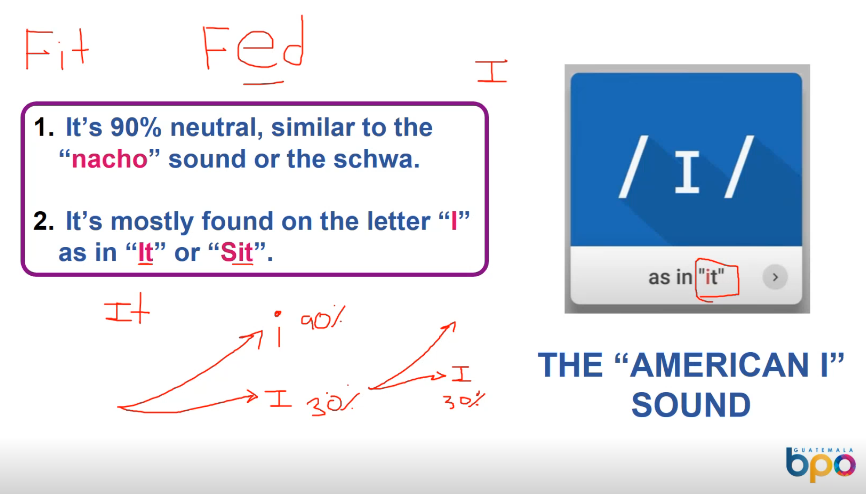
\includegraphics[width=1\textwidth]{images/american_i_portrait.png}
\end{center}

\href{https://drive.google.com/file/d/1BrgaAhXer2RCPNKEfkW6TGB4dQ94Lbvl/view?usp=sharing}{Click here to listen}

\begin{longtable}[c]{||l|l||l|l||}
  \hline
  \textcolor{fancyorange}{Word} & \textcolor{fancyorange}{IPA} & \textcolor{fancyorange}{Word} & \textcolor{fancyorange}{IPA} \\
  \hline
  \textbf{\textcolor{fancyorange}{It}} & \textipa{/'{\textsci}t/} & \textbf{L\textcolor{fancyorange}{i}sten} & \textipa{/'l{\textsci}s.{\textschwa}n/} \\
  \hline
  \textbf{B\textcolor{fancyorange}{i}g} & \textipa{/b{\textsci}g/} & \textbf{F\textcolor{fancyorange}{i}ll} & \textipa{/f{\textsci}l/} \\
  \hline
  \textbf{G\textcolor{fancyorange}{i}ve} & \textipa{/g{\textsci}v/} & \textbf{V\textcolor{fancyorange}{i}s\textcolor{fancyorange}{i}t} & \textipa{/'v{\textsci}z.{\textsci}t/} \\
  \hline
  \textbf{\textcolor{fancyorange}{If}} & \textipa{/'{\textsci}f/} & \textbf{S\textcolor{fancyorange}{i}ster} & \textipa{/'s{\textsci}s.t\textturnr/} \\
  \hline
  \textbf{L\textcolor{fancyorange}{i}ve} & \textipa{/l{\textsci}v/} & \textbf{L\textcolor{fancyorange}{i}st} & \textipa{/l{\textsci}st/} \\
  \hline
  \textbf{D\textcolor{fancyorange}{i}d} & \textipa{/d{\textsci}d/} & \textbf{Ever\textcolor{fancyorange}{y}thing} & \textipa{/'ev.ri.\texttheta{\textsci}\ng/} \\
  \hline
  \textbf{Dr\textcolor{fancyorange}{i}nk} & \textipa{/dr{\textsci}\ng k/} & \textbf{\textcolor{fancyorange}{In}formation} & \textipa{/,{\textsci}n.f{\textschwa}r.'me\textsci.\textesh{\textschwa}n/} \\
  \hline
  \textbf{F\textcolor{fancyorange}{i}t} & \textipa{/f{\textsci}t/} & \textbf{Th\textcolor{fancyorange}{i}nk} & \textipa{/\texttheta{\textsci}\ng k/} \\
  \hline
  \textbf{M\textcolor{fancyorange}{i}ss} & \textipa{/m{\textsci}s/} & \textbf{S\textcolor{fancyorange}{i}ngle} & \textipa{/'s{\textsci}\ng.g{\textschwa}l/} \\
  \hline
  \textbf{K\textcolor{fancyorange}{i}ss} & \textipa{/k{\textsci}s/} & \textbf{\textcolor{fancyorange}{In}terest\textcolor{fancyorange}{e}d} & \textipa{/'{\textsci}n.tr{\textschwa}.st{\textsci}d/} \\
  \hline
  \textbf{K\textcolor{fancyorange}{i}d} & \textipa{/k{\textsci}d/} & \textbf{\textcolor{fancyorange}{In}} & \textipa{/'{\textsci}n/} \\
  \hline
\end{longtable}

\begin{itemize}
  \item[A] \textbf{It's} a beautiful day today, isn't \textbf{it}?
  \item[B] Yeah, you're right. I hope \textbf{it} doesn't rain later because I need to go out. 
\end{itemize}

\begin{itemize}
  \item[A] I \textbf{think} I ate too much cake at the party. I'm feeling a \textbf{bit sick}.
  \item[B] Oh I love cake! What were you \textbf{celebrating}? 
\end{itemize}

\begin{itemize}
  \item[A] So... \textbf{did} you go on a date last week? 
    \item[B] Nope. Honestly, for now I'm \textbf{interested} in being \textbf{single}. And you? 
\end{itemize}

\begin{itemize}
  \item[A] You know, I \textbf{miss} having a summer vacation like when I was a \textbf{kid}.
  \item[B] Yeah, I know what you mean. What \textbf{things did} you use to do on your summer vacations? 
\end{itemize}

\begin{itemize}
  \item[A] \textbf{If} I \textbf{finish} all my assignments today, I'll be free tomorrow.
  \item[B] Great. What are you planning on doing tomorrow?
\end{itemize}

\begin{itemize}
  \item[A] My \textbf{sister} wants to get a loan from the bank just to celebrate her \textbf{birthday}.
  \item[B] Wow, \textbf{it} looks like her \textbf{birthday is} a \textbf{big} deal for her. What do you \textbf{think} about that? 
\end{itemize}

\begin{itemize}
  \item[A] I'm trying to find new music to \textbf{listen} to. Do you have any recommendations?
  \item[B] Well, \textbf{it} depends on the type of music you \textbf{listen} to. Who's your favorite \textbf{artist}? 
\end{itemize}

\begin{itemize}
  \item[A] Do you \textbf{think it} would be better to \textbf{live in} a house or \textbf{in} an apartment?
  \item[B] I'm not sure. Maybe you should \textbf{think} about \textbf{which} one \textbf{is} more expensive. 
\end{itemize}

\begin{itemize}
  \item[A] George, I \textbf{still} have a few \textbf{things} to do from my to-do \textbf{list}. Do you \textbf{think} you can help me \textbf{with} them?
  \item[B] Well, I can \textbf{give it} a shot. What are some of the \textbf{things} you \textbf{still} need to do? 
\end{itemize}

\begin{itemize}
  \item[A] I'm going to be part of a new team, but what \textbf{if} I don't \textbf{fit in}? Any advice?
  \item[B] I'm not sure, but... is \textbf{it} a \textbf{big} deal for you to get along \textbf{with} everyone?
\end{itemize}

\begin{itemize}
  \item[A] So, George, \textbf{did} you like the movie? \textbf{Did it live} up to your expectations?
  \item[B] Honestly, I thought \textbf{it} was just OK, and I wasn't expecting much. How about you?
\end{itemize}

\begin{itemize}
  \item[A] Can I use your card today? I need to \textbf{fill} up my car \textbf{with} gas.
  \item[B] Are you \textbf{kidding} me? You already owe me like Q500. When are you paying me back? 
\end{itemize}





\newpage








\chapter{Consonants}
\section{"TH" sound \textipa{/T/}}
\begin{center}
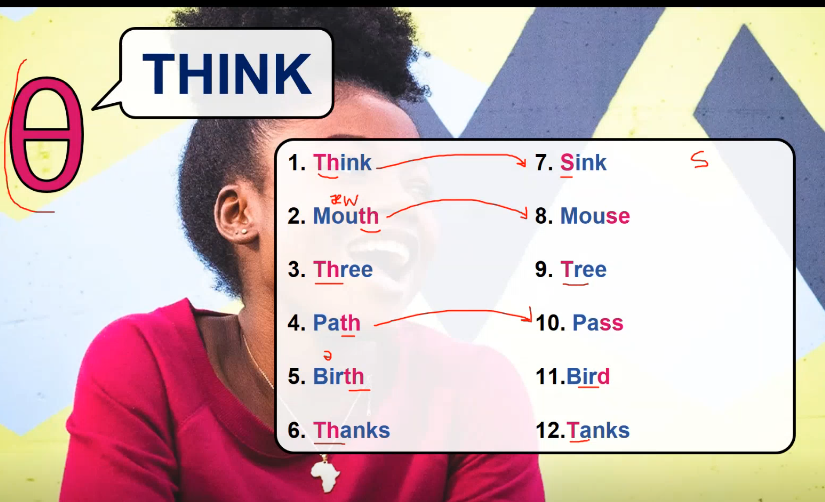
\includegraphics[width=1\textwidth]{images/voiceless_th_portrait.png}
\end{center}

\href{https://drive.google.com/file/d/1Qyxh_48GAe7lFPCOfUzlbQGeDip13594/view?usp=drive_link}{Click here to listen}

\begin{longtable}[c]{||l|l||l|l||}
  \hline
  \textcolor{fancyorange}{Word} & \textcolor{fancyorange}{IPA} &
  \textcolor{fancyorange}{Word} & \textcolor{fancyorange}{IPA} \\
  \hline
  \textbf{\textcolor{fancyorange}{Th}ink} & \textipa{/\texttheta\textsci\ng k/} &
  \textbf{No\textcolor{fancyorange}{th}ing} & \textipa{/'n\textturnv\texttheta.\textsci\ng/} \\
  \textbf{\textcolor{fancyorange}{Th}ought} & \textipa{/\texttheta\textscripta\textlengthmark t/} &
  \textbf{Mon\textcolor{fancyorange}{th}} & \textipa{/m\textturnv n\texttheta/} \\
  \textbf{\textcolor{fancyorange}{Th}ousand} & \textipa{/'\texttheta{\ae}\textupsilon.z\textschwa nd/} &
  \textbf{Mou\textcolor{fancyorange}{th}} & \textipa{/m{\ae}\textupsilon\texttheta/} \\
  \textbf{\textcolor{fancyorange}{Th}umb} & \textipa{/\texttheta\textturnv m/} &
  \textbf{Ear\textcolor{fancyorange}{th}} & \textipa{/\textschwa\textlengthmark\textturnr\texttheta/} \\
  \textbf{\textcolor{fancyorange}{Th}irsty} & \textipa{/'\texttheta\textschwa\textlengthmark\textturnr.sti/} &
  \textbf{Streng\textcolor{fancyorange}{th}} & \textipa{/str\textepsilon\ng\texttheta/} \\
  \textbf{Mara\textcolor{fancyorange}{th}on} & \textipa{/'m\textepsilon\textturnr.\textschwa.\texttheta\textscripta\textlengthmark n/} &
  \textbf{\textcolor{fancyorange}{Th}erapy} & \textipa{/'\texttheta\textepsilon\textturnr.\textschwa.pi/} \\
  \textbf{Heal\textcolor{fancyorange}{th}} & \textipa{/h\textepsilon l\texttheta/} &
  \textbf{\textcolor{fancyorange}{Th}irty} & \textipa{/'\texttheta\textschwa\textlengthmark\textturnr.ti/} \\
  \textbf{Heal\textcolor{fancyorange}{th}y} & \textipa{/'h\textepsilon l.\texttheta i/} &
  \textbf{Tru\textcolor{fancyorange}{th}} & \textipa{/tru\textlengthmark T/} \\
  \textbf{Bir\textcolor{fancyorange}{th}} & \textipa{/b\textschwa\textlengthmark\textturnr\texttheta/} &
  \textbf{Too\textcolor{fancyorange}{th}ache} & \textipa{/'tu\textlengthmark T.e\textsci k/} \\
  \textbf{Bir\textcolor{fancyorange}{th}day} & \textipa{/'b\textschwa\textlengthmark\textturnr\texttheta.de\textsci/} &
  \textbf{Bo\textcolor{fancyorange}{th}} & \textipa{/bo\textupsilon\texttheta/} \\
  \textbf{Some\textcolor{fancyorange}{th}ing} & \textipa{/'s\textturnv m.\texttheta\textsci\ng/} &
  \textbf{Me\textcolor{fancyorange}{th}od} & \textipa{/'m\textepsilon\texttheta.\textschwa d/} \\
  \textbf{Any\textcolor{fancyorange}{th}ing} & \textipa{/'\textepsilon n.i.\texttheta\textsci\ng/} &
  \textbf{Au\textcolor{fancyorange}{th}or} & \textipa{/'\textscripta\textlengthmark.\texttheta\textschwa\textturnr/} \\
  \textbf{Every\textcolor{fancyorange}{th}ing} & \textipa{/'\textepsilon v.ri.\texttheta\textsci\ng/} &
  \textbf{Wor\textcolor{fancyorange}{th}} & \textipa{/w\textschwa\textlengthmark\textturnr\texttheta/} \\
  \hline
\end{longtable}

\begin{enumerate}
  \item I \textbf{think} I know \textbf{everything} now.
  \item Responsability is my biggest \textbf{strength}.
  \item What on \textbf{earth} were you \textbf{thinking}?
  \item \textbf{Thank} you for the \textbf{thirty} bucks you gave me.
  \item Tell me the \textbf{truth} or don't say \textbf{anything}.
  \item Am I \textbf{healthy} enough to run a \textbf{marathon}?
  \item What's your date of \textbf{birth}?
  \item I can't eat \textbf{anything} because of my \textbf{toothache}.
  \item I swear I'm going to pay you back next \textbf{month}.
  \item What is the payment \textbf{method} you used?
  \item I've told you to clean up your mess a \textbf{thousand} times.
  \item Not \textbf{everything} is about you.
  \item Books from that \textbf{author} are \textbf{worth} a lot of money.
  \item I'll \textbf{think} about you when I go to \textbf{therapy}.
  \item I can't believe \textbf{both} of you \textbf{thought} this was a good idea.
\end{enumerate}


\newpage







\section{"TH" sound \textipa{/ð/} (as in \textit{that}, \textit{those}, \textit{they})}
\begin{center}
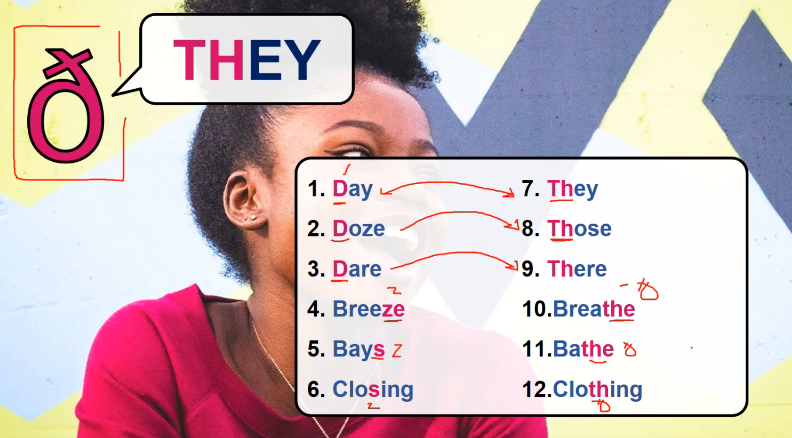
\includegraphics[width=1\textwidth]{images/voiced_th_portrait.png}
\end{center}

\href{https://drive.google.com/file/d/1XmUZs4md19kMjeZFluzftm0_2KcIrsU3/view?usp=drive_link}{Click here to listen}

\begin{longtable}[c]{||l|l||l|l||}
  \hline
  \textcolor{fancyorange}{Word} & \textcolor{fancyorange}{IPA} & \textcolor{fancyorange}{Word} & \textcolor{fancyorange}{IPA} \\
  \hline
  \textbf{\textcolor{fancyorange}{Th}at} & \textipa{'{\dh}{\ae}t} & \textbf{Toge\textcolor{fancyorange}{th}er} & \textipa{t\textschwa'g\textepsilon{\dh}\textschwa\textturnr} \\
  \textbf{\textcolor{fancyorange}{Th}an} & \textipa{'{\dh}{\ae}n} & \textbf{Ei\textcolor{fancyorange}{th}er} & \textipa{'i{\dh}\textturnr} \\
  \textbf{\textcolor{fancyorange}{Th}ey} & \textipa{'{\dh}e\textsci} & \textbf{\textcolor{fancyorange}{Th}ose} & \textipa{'{\dh}o\textupsilon z} \\
  \textbf{Fa\textcolor{fancyorange}{th}er} & \textipa{'f\textscripta{\dh}\textschwa\textturnr} & \textbf{Lea\textcolor{fancyorange}{th}er} & \textipa{'l\textepsilon{\dh}\textschwa\textturnr} \\
  \textbf{Mo\textcolor{fancyorange}{th}er} & \textipa{'m\textturnv{\dh}\textschwa\textturnr} & \textbf{O\textcolor{fancyorange}{th}er} & \textipa{'\textturnv{\dh}\textschwa\textturnr} \\
  \textbf{Bro\textcolor{fancyorange}{th}er} & \textipa{'b\textturnr\textturnv{\dh}\textschwa\textturnr} & \textbf{Ano\textcolor{fancyorange}{th}er} & \textipa{\textschwa'n\textturnv{\dh}\textschwa\textturnr} \\
  \textbf{Fea\textcolor{fancyorange}{th}er} & \textipa{'f\textepsilon{\dh}\textschwa\textturnr} & \textbf{Brea\textcolor{fancyorange}{th}e} & \textipa{'bri\textlengthmark{\dh}} \\
  \textbf{Wea\textcolor{fancyorange}{th}er} & \textipa{'w\textepsilon{\dh}\textschwa\textturnr} & \textbf{(Even) Though} & \textipa{'{\dh}o\textupsilon} \\
  \textbf{Ga\textcolor{fancyorange}{th}er} & \textipa{'g{\ae}{\dh}\textschwa\textturnr} & \textbf{Clo\textcolor{fancyorange}{th}ing} & \textipa{'klo\textupsilon{\dh}\textsci\ng} \\
  \textbf{Ra\textcolor{fancyorange}{th}er} & \textipa{'\textturnr{\ae}{\dh}\textschwa\textturnr} & \textbf{Smoo\textcolor{fancyorange}{th}} & \textipa{'smu\textlengthmark{\dh}} \\
  \hline
\end{longtable}

Even \textbf{though the weather} has been very cold \textbf{these} days,
our family is going to get \textbf{together} for dinner. It's just 
\textbf{another} tradition \textbf{that} we have.
\\\\
First, our \textbf{father} prepares some hot chocolate for 
everybody. \textbf{Then} our \textbf{mother} bakes some delicious
cookies. And, believe it or not, my \textbf{brother} cooks some
delicious pizza.
\\\\
We \textbf{gather} around the fireplace in our living room and we 
\textbf{either} play board games or watch a movie. We do \textbf{other}
activities like telling scary stories or playing Pictionary.
\\\\
I \textbf{rather} play board games because it's more interactive 
and we laugh more, but watching a movie is also a good 
option.
\\\\
When the \textbf{weather} gets better, we go out and \textbf{breathe} the
fresh air. \textbf{These} are some of the moments I always
appreciate, and \textbf{whether} I'm young or old, I will always 
remember \textbf{them}.











\newpage







\section{"SH" sound \textipa{/\textesh/}}
\begin{center}
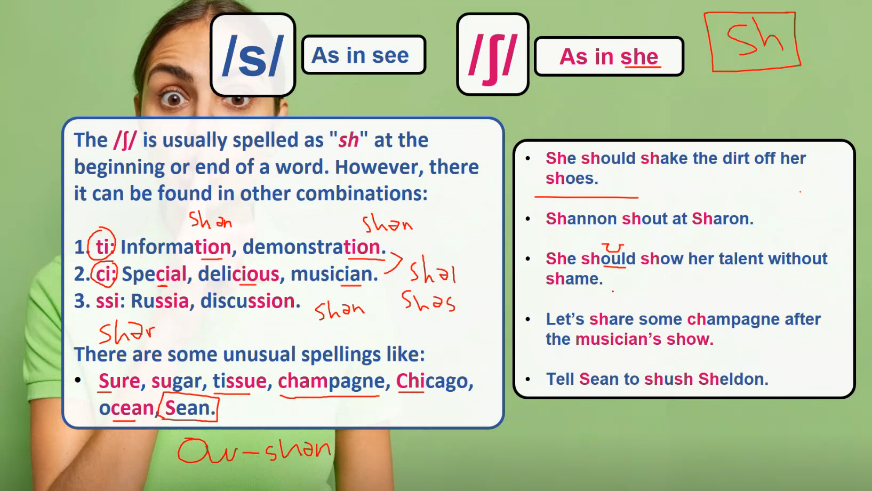
\includegraphics[width=1\textwidth]{images/sh_portrait.png}
\end{center}

\href{https://drive.google.com/file/d/18J6AvoCQcRX4x2EfFuk6YyZnvlKzgbea/view?usp=drive_link}{Click here to listen}

% \begin{longtable}[c]{||l|l||}
%   \hline
%   \textcolor{fancyorange}{Word} & \textcolor{fancyorange}{IPA} \\
%   \hline
%   Invitation       & \textipa{/\,\textsci nv\textsci'te\textlengthmark\textesh\textschwa n/} \\
%   Solution         & \textipa{/s\textschwa'lu\textlengthmark\textesh\textschwa n/} \\
%   Beneficial       & \textipa{/b\textepsilon n\textschwa'f\textsci\textesh\textschwa l/} \\
%   Artificial       & \textipa{/\textscripta\textlengthmark rt\textschwa'f\textsci\textesh\textschwa l/} \\
%   Financial        & \textipa{/fa\textsci'n\ae n\textesh\textschwa l/} \\
%   Official         & \textipa{/\textschwa'f\textsci\textesh\textschwa l/} \\
%   Special          & \textipa{/'sp\textepsilon\textesh\textschwa l/} \\
%   Social           & \textipa{/'so\textlengthmark\textesh\textschwa l/} \\
%   Suspicious       & \textipa{/s\textschwa 'sp\textsci \textesh\textschwa s/} \\
%   Delicious        & \textipa{/d\textsci'l\textsci\textesh\textschwa s/} \\
%   Precious         & \textipa{/'pr\textepsilon\textesh\textschwa s/} \\
%   Registration     & \textipa{/r\textepsilon d\textyogh\textsci'st\textlengthmark\textesh\textschwa n/} \\
%   Identification   & \textipa{/a\textsci,d\textsci f\textsci'ke\textlengthmark\textesh\textschwa n/} \\
%   Administration   & \textipa{/\textschwa d'm\textsci n\textesh\textschwa 't\textlengthmark\textesh\textschwa n/} \\
%   Congratulations  & \textipa{/k\textschwa n,gr\ae t\textesh\textschwa'le\textlengthmark\textesh\textschwa n z/} \\
%   Investigation    & \textipa{/,\textsci n,v\textepsilon s,t\textsci'ge\textlengthmark\textesh\textschwa n/} \\
%   Communication    & \textipa{/k\textschwa,mju'n\textsci ke\textlengthmark\textesh\textschwa n/} \\
%   Direction        & \textipa{/da\textsci'r\textepsilon k\textesh\textschwa n/} \\
%   Pronunciation    & \textipa{/pr\textschwa n\textsci\textlengthmark'si e\textscripta\textesh\textschwa n/} \\
%   Discussion       & \textipa{/d\textsci'sk\textturnv\textesh\textschwa n/} \\
%   Expression       & \textipa{/ek'spr\textepsilon\textesh\textschwa n/} \\
%   Obsession        & \textipa{/ \textschwa b 's \textepsilon \textesh \textschwa n/} \\
%   Mission          & \textipa{/'m\textsci\textesh\textschwa n/} \\
%   Passion          & \textipa{/'p\ae\textesh\textschwa n/} \\
%   Session          & \textipa{/'s\textepsilon\textesh\textschwa n/} \\
%   Condition        & \textipa{/k\textschwa n'd\textsci\textesh\textschwa n/} \\
%   Repetition       & \textipa{/r\textepsilon p\textsci't\textsci\textesh\textschwa n/} \\
%   Retention        & \textipa{/r\textsci't\textepsilon n\textesh\textschwa n/} \\
%   Medication       & \textipa{/m\textepsilon d\textsci'ke\textlengthmark\textesh\textschwa n/} \\
%   Mention          & \textipa{/'m\textsci\textesh\textschwa n/} \\
%   Nation           & \textipa{/'ne\textsci\textesh\textschwa n/} \\
%   Compensation     & \textipa{/k\textschwa m p\textschwa n'se\textsci\textesh\textschwa n/} \\
%   Issue            & \textipa{/'\textsci\textesh\textschwa/} \\
%   Machine          & \textipa{/m\textschwa'\textesh\textsci\textlengthmark n/} \\
%   Michigan         & \textipa{/'m\textsci\textesh\textsci g\textsci n/} \\
%   Lotion           & \textipa{/'lo\textlengthmark\textesh\textschwa n/} \\
%   Chef             & \textipa{/'\textesh\textepsilon f/} \\
%   Ocean            & \textipa{/'o\textlengthmark\textesh\textschwa n/} \\
%   Patient          & \textipa{/'pe\textsci\textesh\textschwa n/} \\
%   Patience         & \textipa{/'pe\textsci\textesh\textschwa ns/} \\
%   Sure             & \textipa{/'\textesh\textupsilon r/} \\
%   Promotion        & \textipa{/pr\textschwa 'mo\textlengthmark \textesh \textschwa n/} \\
%   Appreciate       & \textipa{/\textschwa 'pri \textesh i \textlengthmark e \textsci t/} \\
%   Pressure         & \textipa{/'pr\textepsilon\textesh\textschwa r/} \\
%   Mention          & \textipa{/'m\textsci\textesh\textschwa n/} \\
%   Conversation     & \textipa{/k\textschwa nv\textschwa 'se\textlengthmark\textesh\textschwa n/} \\
%   Dedication       & \textipa{/d\textepsilon d\textsci'ke\textlengthmark\textesh\textschwa n/} \\
%   \hline
% \end{longtable}

\begin{longtable}[c]{||l|l||l|l||}
  \hline
  \textcolor{fancyorange}{Word} & \textcolor{fancyorange}{IPA} & \textcolor{fancyorange}{Word} & \textcolor{fancyorange}{IPA} \\
  \hline
  \textbf{Invita\textcolor{fancyorange}{ti}on}       & \textipa{/\,\textsci nv\textsci'te\textlengthmark\textesh\textschwa n/} & \textbf{Se\textcolor{fancyorange}{ss}ion}          & \textipa{/'s\textepsilon\textesh\textschwa n/} \\
  \textbf{Solu\textcolor{fancyorange}{ti}on}         & \textipa{/s\textschwa'lu\textlengthmark\textesh\textschwa n/} & \textbf{Condi\textcolor{fancyorange}{ti}on}        & \textipa{/k\textschwa n'd\textsci\textesh\textschwa n/} \\
  \textbf{Benefi\textcolor{fancyorange}{ci}al}       & \textipa{/b\textepsilon n\textschwa'f\textsci\textesh\textschwa l/} & \textbf{Repe\textcolor{fancyorange}{ti}tion}       & \textipa{/r\textepsilon p\textsci't\textsci\textesh\textschwa n/} \\
  \textbf{Artifi\textcolor{fancyorange}{ci}al}        & \textipa{/\textscripta\textlengthmark rt\textschwa'f\textsci\textesh\textschwa l/} & \textbf{Re\textcolor{fancyorange}{ti}ntion}        & \textipa{/r\textsci't\textepsilon n\textesh\textschwa n/} \\
  \textbf{Finan\textcolor{fancyorange}{ci}al}        & \textipa{/fa\textsci'n\ae n\textesh\textschwa l/} & \textbf{Medica\textcolor{fancyorange}{ti}on}       & \textipa{/m\textepsilon d\textsci'ke\textlengthmark\textesh\textschwa n/} \\
  \textbf{Offi\textcolor{fancyorange}{ci}al}           & \textipa{/\textschwa'f\textsci\textesh\textschwa l/} & \textbf{Men\textcolor{fancyorange}{ti}on}          & \textipa{/'m\textsci\textesh\textschwa n/} \\
  \textbf{Spe\textcolor{fancyorange}{ci}al}          & \textipa{/'sp\textepsilon\textesh\textschwa l/} & \textbf{Na\textcolor{fancyorange}{ti}on}           & \textipa{/'ne\textsci\textesh\textschwa n/} \\
  \textbf{So\textcolor{fancyorange}{ci}al}           & \textipa{/'so\textlengthmark\textesh\textschwa l/} & \textbf{Compensa\textcolor{fancyorange}{ti}on}     & \textipa{/k\textschwa m p\textschwa n'se\textsci\textesh\textschwa n/} \\
  \textbf{Suspi\textcolor{fancyorange}{ci}ous}       & \textipa{/s\textschwa 'sp\textsci \textesh\textschwa s/} & \textbf{I\textcolor{fancyorange}{ss}ue}            & \textipa{/'\textsci\textesh\textschwa/} \\
  \textbf{Deli\textcolor{fancyorange}{ci}ous}        & \textipa{/d\textsci'l\textsci\textesh\textschwa s/} & \textbf{Ma\textcolor{fancyorange}{ch}ine}          & \textipa{/m\textschwa'\textesh\textsci\textlengthmark n/} \\
  \textbf{Pre\textcolor{fancyorange}{ci}ous}         & \textipa{/'pr\textepsilon\textesh\textschwa s/} & \textbf{Mi\textcolor{fancyorange}{ch}igan}         & \textipa{/'m\textsci\textesh\textsci g\textsci n/} \\
  \textbf{Registra\textcolor{fancyorange}{ti}on}     & \textipa{/r\textepsilon d\textyogh\textsci'st\textlengthmark\textesh\textschwa n/} & \textbf{Lo\textcolor{fancyorange}{ti}on}           & \textipa{/'lo\textlengthmark\textesh\textschwa n/} \\
  \textbf{Identifica\textcolor{fancyorange}{ti}on}    & \textipa{/a\textsci,d\textsci f\textsci'ke\textlengthmark\textesh\textschwa n/} & \textbf{\textcolor{fancyorange}{Ch}ef}             & \textipa{/'\textesh\textepsilon f/} \\
  \textbf{Administra\textcolor{fancyorange}{ti}on}   & \textipa{/\textschwa d'm\textsci n\textesh\textschwa 't\textlengthmark\textesh\textschwa n/} & \textbf{O\textcolor{fancyorange}{ce}an}            & \textipa{/'o\textlengthmark\textesh\textschwa n/} \\
  \textbf{Congra\textcolor{fancyorange}{tu}lations}  & \textipa{/k\textschwa n,gr\ae t\textesh\textschwa'le\textlengthmark\textesh\textschwa n z/} & \textbf{Pa\textcolor{fancyorange}{ti}ent}          & \textipa{/'pe\textsci\textesh\textschwa n/} \\
  \textbf{Investiga\textcolor{fancyorange}{ti}on}    & \textipa{/,\textsci n,v\textepsilon s,t\textsci'ge\textlengthmark\textesh\textschwa n/} & \textbf{Pa\textcolor{fancyorange}{ti}ence}         & \textipa{/'pe\textsci\textesh\textschwa ns/} \\
  \textbf{Communica\textcolor{fancyorange}{ti}on}    & \textipa{/k\textschwa,mju'n\textsci ke\textlengthmark\textesh\textschwa n/} & \textbf{\textcolor{fancyorange}{Sh}ure}            & \textipa{/'\textesh\textupsilon r/} \\
  \textbf{Direc\textcolor{fancyorange}{ti}on}        & \textipa{/da\textsci'r\textepsilon k\textesh\textschwa n/} & \textbf{Promo\textcolor{fancyorange}{ti}on}        & \textipa{/pr\textschwa 'mo\textlengthmark \textesh \textschwa n/} \\
  \textbf{Pronuncia\textcolor{fancyorange}{ti}on}    & \textipa{/pr\textschwa n\textsci\textlengthmark'si e\textscripta\textesh\textschwa n/} & \textbf{Appre\textcolor{fancyorange}{ci}ate}        & \textipa{/\textschwa 'pri \textesh i \textlengthmark e \textsci t/} \\
  \textbf{Discu\textcolor{fancyorange}{ss}ion}       & \textipa{/d\textsci'sk\textturnv\textesh\textschwa n/} & \textbf{Pre\textcolor{fancyorange}{ss}ure}         & \textipa{/'pr\textepsilon\textesh\textschwa r/} \\
  \textbf{Expre\textcolor{fancyorange}{ss}ion}       & \textipa{/ek'spr\textepsilon\textesh\textschwa n/} & \textbf{Men\textcolor{fancyorange}{ti}on}          & \textipa{/'m\textsci\textesh\textschwa n/} \\
  \textbf{Obse\textcolor{fancyorange}{ss}ion}        & \textipa{/ \textschwa b 's \textepsilon \textesh \textschwa n/} & \textbf{Conversa\textcolor{fancyorange}{ti}on}     & \textipa{/k\textschwa nv\textschwa 'se\textlengthmark\textesh\textschwa n/} \\
  \textbf{Mi\textcolor{fancyorange}{ss}ion}          & \textipa{/'m\textsci\textesh\textschwa n/} & \textbf{Dedica\textcolor{fancyorange}{ti}on}       & \textipa{/d\textepsilon d\textsci'ke\textlengthmark\textesh\textschwa n/} \\
  \textbf{Pa\textcolor{fancyorange}{ss}ion}          & \textipa{/'p\ae\textesh\textschwa n/} &                  &  \\
  \hline
\end{longtable}

\begin{itemize}
  \item I got an \textbf{invita\textcolor{fancyorange}{ti}on}.
  \item What's the \textbf{solu\textcolor{fancyorange}{ti}on}?
  \item We have \textbf{finan\textcolor{fancyorange}{ci}al} problems.
  \item Let's have a \textbf{conversa\textcolor{fancyorange}{ti}on}.
  \item Follow the \textbf{registra\textcolor{fancyorange}{ti}on} process.
  \item Great \textbf{pronuncia\textcolor{fancyorange}{ti}on}.
  % A new expression.
  \item A new \textbf{expre\textcolor{fancyorange}{ss}ion}.
  \item I have \textbf{reten\textcolor{fancyorange}{ti}on} skills.
  \item \textbf{\textcolor{fancyorange}{Sh}e's} on \textbf{medica\textcolor{fancyorange}{ti}on}.
  \item There's a new \textbf{i\textcolor{fancyorange}{ss}ue}.
  \item He wants some \textbf{compensa\textcolor{fancyorange}{ti}on}.
  \item Thank you for your \textbf{pa\textcolor{fancyorange}{cie}nce}, I \textbf{appre\textcolor{fancyorange}{ci}ate} it.
  \item I heard you got a \textbf{promo\textcolor{fancyorange}{ti}on}. \textbf{Congratula\textcolor{fancyorange}{ti}ons}.
  \item Don't \textbf{men\textcolor{fancyorange}{ti}on} it.
\end{itemize}

% \begin{tabular}{||l|l|p{3.5cm}||}
%   \hline
%   \textbf{Sound} & \textbf{IPA Symbol} & \textbf{TIPA command (for \textbackslash textipa\{\})} \\
%   \hline\hline

%   \multicolumn{3}{||c||}{\textbf{Consonants}} \\
%   \hline
%   Voiceless bilabial plosive & \textipa{p} & \texttt{p} \\
%   Voiced bilabial plosive & \textipa{b} & \texttt{b} \\
%   Voiceless alveolar plosive & \textipa{t} & \texttt{t} \\
%   Voiced alveolar plosive & \textipa{d} & \texttt{d} \\
%   Voiceless velar plosive & \textipa{k} & \texttt{k} \\
%   Voiced velar plosive & \textipa{g} & \texttt{g} \\
%   Bilabial nasal & \textipa{m} & \texttt{m} \\
%   Alveolar nasal & \textipa{n} & \texttt{n} \\
%   Velar nasal & \textipa{\ng} & \texttt{ng} \\
%   Voiceless labiodental fricative & \textipa{f} & \texttt{f} \\
%   Voiced labiodental fricative & \textipa{v} & \texttt{v} \\
%   Voiceless dental fricative & \textipa{\texttheta} & \texttt{texttheta} \\
%   Voiced dental fricative & \textipa{\dh} & \texttt{dh} \\
%   Voiceless alveolar fricative & \textipa{s} & \texttt{s} \\
%   Voiced alveolar fricative & \textipa{z} & \texttt{z} \\
%   Voiceless postalveolar fricative & \textipa{\textesh} & \texttt{textesh} \\
%   Voiced postalveolar fricative & \textipa{\textyogh} & \texttt{textyogh} \\
%   Voiceless glottal fricative & \textipa{h} & \texttt{h} \\
%   Voiceless postalveolar affricate & \textipa{t\textesh} & \texttt{ttextesh} \\
%   Voiced postalveolar affricate & \textipa{d\textyogh} & \texttt{dtextyogh} \\
%   Alveolar approximant & \textipa{\textturnr} & \texttt{textturnr} \\
%   Palatal approximant & \textipa{j} & \texttt{j} \\
%   Labio-velar approximant & \textipa{w} & \texttt{w} \\
%   Alveolar lateral approximant & \textipa{l} & \texttt{l} \\
%   \hline

%   \multicolumn{3}{||c||}{\textbf{Vowels}} \\
%   \hline
%   Close front unrounded vowel & \textipa{i} & \texttt{i} \\
%   Near-close near-front unrounded vowel & \textipa{\textsci} & \texttt{textsci} \\
%   Close-mid front unrounded vowel & \textipa{e} & \texttt{e} \\
%   Open-mid front unrounded vowel & \textipa{\textepsilon} & \texttt{textepsilon} \\
%   Near-open front unrounded vowel & \textipa{{\ae}} & \texttt{{\ae}} \\
%   Mid central vowel (schwa) & \textipa{\textschwa} & \texttt{textschwa} \\
%   Open-mid back unrounded vowel & \textipa{\textturnv} & \texttt{textturnv} \\
%   Near-close near-back rounded vowel & \textipa{\textupsilon} & \texttt{textupsilon} \\
%   Close back rounded vowel & \textipa{u} & \texttt{u} \\
%   Open back unrounded vowel & \textipa{\textscripta} & \texttt{textscripta} \\
%   Open-mid back rounded vowel & \textipa{\textopeno} & \texttt{textopeno} \\
%   \hline

%   \multicolumn{3}{||c||}{\textbf{Diphthongs (as combinations)}} \\
%   \hline
%   \textipa{/e\textsci/} (as in face) & \textipa{e\textsci} & \texttt{e textsci} \\
%   \textipa{/{\ae}\textsci/} (as in price) & \textipa{{\ae}\textsci} & \texttt{{\ae} textsci} \\
%   \textipa{/\textopeno\textsci/} (as in choice) & \textipa{\textopeno\textsci} & \texttt{textopeno textsci} \\
%   \textipa{/{\ae}\textupsilon/} (as in mouth) & \textipa{{\ae}\textupsilon} & \texttt{{\ae} textupsilon} \\
%   \textipa{/o\textupsilon/} (as in goat) & \textipa{o\textupsilon} & \texttt{o textupsilon} \\
%   \hline  
% \end{tabular}

\newpage







% ONLY TIPA CODE IS ALLOWED IN THIS FILE
% DO NOT ADD ANYTHING ELSE
\section{"ZH" Sound (\textipa{/\textyogh/})}
\begin{center}
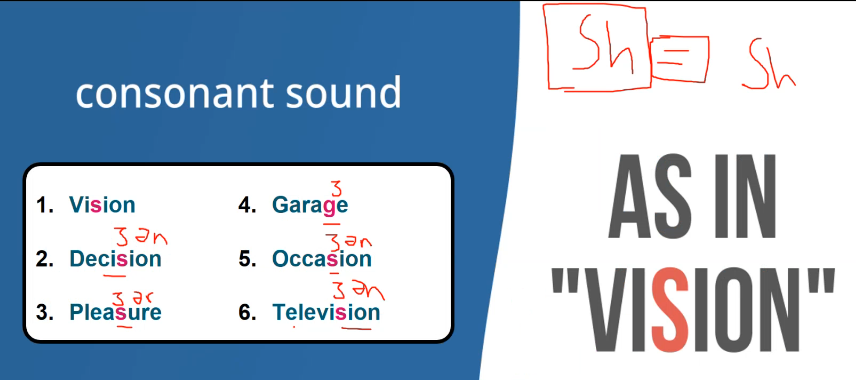
\includegraphics[width=1\textwidth]{images/zh_portraint.png}
\end{center}

\href{https://drive.google.com/file/d/1J5EL2Z3BKZqDA29fe09p-RAgaJgx5Y2W/view?usp=sharing}{Click here to listen}

\begin{longtable}[c]{||l|l||l|l||}
  \hline
  \textcolor{fancyorange}{Word} & \textcolor{fancyorange}{IPA} & \textcolor{fancyorange}{Word} & \textcolor{fancyorange}{IPA} \\
  \hline
  \textbf{Vi\textcolor{fancyorange}{s}ion}            & \textipa{/'v\textsci\textyogh\textschwa n/} & \textbf{Lei\textcolor{fancyorange}{s}ure}           & \textipa{/'li\textyogh\textschwa\textturnr/} \\
  \textbf{Deci\textcolor{fancyorange}{s}ion}          & \textipa{/d\textsci's\textsci\textyogh\textschwa n/} & \textbf{Occa\textcolor{fancyorange}{s}ion}          & \textipa{/\textschwa'ke\textsci\textyogh\textschwa n/} \\
  \textbf{Mea\textcolor{fancyorange}{s}ure}           & \textipa{/'m\textepsilon\textyogh\textschwa\textturnr/} & \textbf{Preci\textcolor{fancyorange}{s}ion}         & \textipa{/pr\textsci's\textsci\textyogh\textschwa n/} \\
  \textbf{U\textcolor{fancyorange}{s}ual}             & \textipa{/'ju\textyogh\textschwa l/} & \textbf{Televi\textcolor{fancyorange}{s}ion}        & \textipa{/'t\textepsilon l\textschwa v\textsci\textyogh\textschwa n/} \\
  \textbf{Massa\textcolor{fancyorange}{ge}}           & \textipa{/m\textschwa's\textopeno\textyogh/} & \textbf{Ver\textcolor{fancyorange}{s}ion}           & \textipa{/'v\textturnv\textlengthmark\textturnr\textyogh\textschwa n/} \\
  \textbf{Bei\textcolor{fancyorange}{ge}}             & \textipa{/be\textsci\textyogh/} & \textbf{Confu\textcolor{fancyorange}{s}ion}         & \textipa{/k\textschwa n'fju\textyogh\textschwa n/} \\
  \textbf{A\textcolor{fancyorange}{s}ia}              & \textipa{/'e\textsci\textyogh\textschwa/} & \textbf{Illu\textcolor{fancyorange}{s}ion}          & \textipa{/\textsci'lu\textyogh\textschwa n/} \\
  \textbf{Conclu\textcolor{fancyorange}{s}ion}        & \textipa{/k\textschwa n'klu\textyogh\textschwa n/} & \textbf{Supervi\textcolor{fancyorange}{s}ion}       & \textipa{/,su\textschwa p\textturnr'v\textsci\textyogh\textschwa n/} \\
  \textbf{Divi\textcolor{fancyorange}{s}ion}          & \textipa{/d\textsci'v\textsci\textyogh\textschwa n/} & \textbf{Trea\textcolor{fancyorange}{s}ure}          & \textipa{/'tr\textepsilon\textyogh\textschwa\textturnr/} \\
  \textbf{Gara\textcolor{fancyorange}{ge}}            & \textipa{/g\textschwa'r\textopeno\textyogh/} & \textbf{\textcolor{fancyorange}{G}enre}             & \textipa{/'\textyogh\textscripta n.\textturnr\textschwa/} \\
  \textbf{Ple\textcolor{fancyorange}{s}ure}          & \textipa{/'pl\textepsilon\textyogh\textschwa\textturnr/} & \textbf{U\textcolor{fancyorange}{s}ually}           & \textipa{/'ju\textlengthmark.\textyogh u.\textschwa l\textsci/} \\
  \hline
\end{longtable}
% numbered list

\begin{enumerate}
  \item I have this \textbf{vi\textcolor{fancyorange}{si}on} of starting my own business one day, you know.
  \item It was such a \textbf{plea\textcolor{fancyorange}{su}re} meeting you today!
  \item Have you made a \textbf{deci\textcolor{fancyorange}{si}on} about the job offer?
  \item I'm in total \textbf{confu\textcolor{fancyorange}{si}on} right now. I don't understand this assignment.
  \item Do you \textbf{u\textcolor{fancyorange}{su}ally} watch a lot of \textbf{televi\textcolor{fancyorange}{si}on}?
  \item Have you heard the acusting \textbf{ver\textcolor{fancyorange}{si}on} of this song?
  \item I'll check it out. I love when songs have different \textbf{ver\textcolor{fancyorange}{si}ons}.
  \item What's your favorite movie \textbf{gen\textcolor{fancyorange}{re}}?
  \item You should take it to the \textbf{gara\textcolor{fancyorange}{ge}} before it gets worse.
  \item Do you \textbf{u\textcolor{fancyorange}{su}ally} wake up this early?
  \item Hey, do you want your \textbf{u\textcolor{fancyorange}{su}al} coffee order?
  \item Of course! It's a special \textbf{occa\textcolor{fancyorange}{si}on}.
  \item Have you ever been to \textbf{A\textcolor{fancyorange}{si}a}?
  \item I really need a \textbf{massa\textcolor{fancyorange}{ge}}. My back is killing me.
  \item Can you work on this project without \textbf{supervi\textcolor{fancyorange}{si}on}?
  \item What \textbf{gen\textcolor{fancyorange}{re}} are you in the mood for ?
  \item I finally made a \textbf{deci\textcolor{fancyorange}{si}on} about the apartment. 
\end{enumerate}

\newpage







\section{"CH" sound as in "chair" \textipa{/t\textesh/}}
\begin{center}
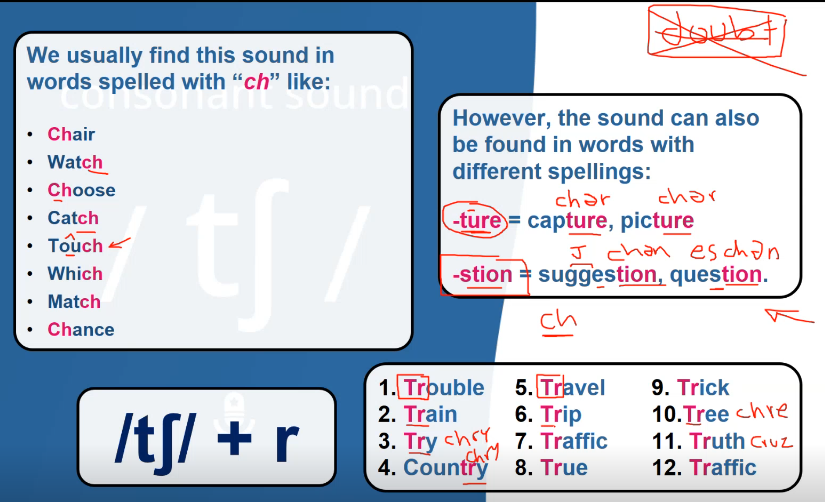
\includegraphics[width=1\textwidth]{images/ch_portrait.png}
\end{center}

\href{https://drive.google.com/file/d/1iXGD0OdMNuyyw2AJ0a7Dr2jUlRgxtkmr/view?usp=drive_link}{Click here to listen}

\begin{longtable}[c]{||l|l||l|l||}
  \hline
  \textcolor{fancyorange}{Word} & \textcolor{fancyorange}{IPA} & \textcolor{fancyorange}{Word} & \textcolor{fancyorange}{IPA} \\
  \hline
  \textbf{Ar\textcolor{fancyorange}{ch}itecture} & \textipa{/'\textscripta\textlengthmark\textturnr.k\textschwa.t\textschwa.t\textesh\textschwa\textturnr/} & \textbf{Ques\textcolor{fancyorange}{ti}on} & \textipa{/'kw\textepsilon s.t\textesh\textschwa n/} \\
  \textbf{Tempera\textcolor{fancyorange}{t}ure} & \textipa{/'t\textepsilon m.p\textschwa\textturnr.\textschwa.t\textesh\textschwa\textturnr/} & \textbf{\textcolor{fancyorange}{Ch}ildish} & \textipa{/'t\textesh{\ae}\textsci l.d\textsci\textesh/} \\
  \textbf{I\textcolor{fancyorange}{tch}} & \textipa{/\textsci t\textesh/} & \textbf{Exhaus\textcolor{fancyorange}{ti}on} & \textipa{/\textsci g'z\textscripta\textlengthmark s.t\textesh\textschwa n/} \\
  \textbf{Swi\textcolor{fancyorange}{tch}} & \textipa{/sw\textsci t\textesh/} & \textbf{Pos\textcolor{fancyorange}{t}ure} & \textipa{/'p\textscripta\textlengthmark s.t\textesh\textschwa\textturnr/} \\
  \textbf{Cul\textcolor{fancyorange}{t}ure} & \textipa{/'k\textturnv l.t\textesh\textschwa\textturnr/} & \textbf{Sta\textcolor{fancyorange}{t}ue} & \textipa{/'st{\ae}t\textesh.u\textlengthmark/} \\
  \textbf{Struc\textcolor{fancyorange}{t}ure} & \textipa{/'str\textturnv k.t\textesh\textschwa\textturnr/} & \textbf{Ges\textcolor{fancyorange}{t}ure} & \textipa{/'d\textyogh\textepsilon s.t\textesh\textschwa\textturnr/} \\
  \textbf{Furni\textcolor{fancyorange}{t}ure} & \textipa{/'f\textschwa\textlengthmark\textturnr.n\textschwa.t\textesh\textschwa\textturnr/} & \textbf{A\textcolor{fancyorange}{ch}ievement} & \textipa{/\textschwa't\textesh i\textlengthmark v.m\textschwa nt/} \\
  \textbf{Adven\textcolor{fancyorange}{t}ure} & \textipa{/\textschwa d'v\textepsilon n.t\textesh\textschwa\textturnr/} & \textbf{For\textcolor{fancyorange}{t}une} & \textipa{/'f\textopeno\textlengthmark\textturnr.t\textesh un/} \\
  \textbf{Signa\textcolor{fancyorange}{t}ure} & \textipa{/'s\textsci g.n\textschwa.t\textesh\textschwa\textturnr/} & \textbf{Unfor\textcolor{fancyorange}{t}unately} & \textipa{/,\textturnv n'f\textopeno\textlengthmark\textturnr.t\textesh n.\textschwa t.li/} \\
  \textbf{Crea\textcolor{fancyorange}{t}ure} & \textipa{/'kri\textlengthmark.t\textesh\textschwa\textturnr/} & \textbf{Chris\textcolor{fancyorange}{ti}an} & \textipa{/'kr\textsci s.t\textesh\textschwa n/} \\
  \textbf{Frac\textcolor{fancyorange}{t}ure} & \textipa{/'fr{\ae}k.t\textesh\textschwa\textturnr/} & \textbf{Country} & \textipa{/'k\textturnv n.tri/} \\
  \textbf{Imma\textcolor{fancyorange}{t}ure} & \textipa{/,\textsci m.\textschwa't\textesh\textupsilon\textturnr/} & \textbf{True} & \textipa{/tru\textlengthmark/} \\
  \textbf{Fu\textcolor{fancyorange}{t}ure} & \textipa{/'fju\textlengthmark.t\textesh\textschwa\textturnr/} & \textbf{Traffic} & \textipa{/'tr{\ae}f.\textsci k/} \\
  \textbf{Pic\textcolor{fancyorange}{t}ure} & \textipa{/'p\textsci k.t\textesh\textschwa\textturnr/} & \textbf{Trip} & \textipa{/tr\textsci p/} \\
  \textbf{Fea\textcolor{fancyorange}{t}ure} & \textipa{/'fi\textlengthmark.t\textesh\textschwa\textturnr/} & \textbf{Travel} & \textipa{/'tr{\ae}v.\textschwa l/} \\
  \textbf{Na\textcolor{fancyorange}{t}ure} & \textipa{/'ne\textsci.t\textesh\textschwa\textturnr/} & \textbf{Si\textcolor{fancyorange}{t}uation} & \textipa{/,\textsci t\textesh.u'e\textsci.\textesh\textschwa n/} \\
  \textbf{Ma\textcolor{fancyorange}{t}ure} & \textipa{/m\textschwa't\textesh\textupsilon\textturnr/} & \textbf{\textcolor{fancyorange}{Ch}ocolate} & \textipa{/'t\textesh\textscripta\textlengthmark k.l\textschwa t/} \\
  \hline  
\end{longtable}

\begin{itemize}
  \item[A] What's the \textbf{temperature} like outside?
  \item[B] It's colder than I expected, so it's a good idea to bring a sweater. Are you planning to go out? 
\end{itemize}

\begin{itemize}
  \item[A] Have you ever been on a real \textbf{adventure}?
  \item[B] I went on a camping \textbf{trip} in the mountains last year. It was incredible! How about you? 
\end{itemize}

\begin{itemize}
  \item[A] What do you love most about \textbf{travelling}?
  \item[B] Experiencing new \textbf{cultures} and \textbf{trying traditional} food. Would you like to explore a specific \textbf{country} or \textbf{culture}?  
\end{itemize}

\begin{itemize}
  \item[A] Did you get tickets for the concert?
  \item[B] \textbf{Unfortunately}, it was sold out by the time I \textbf{checked}. Do you want to do something else?
\end{itemize}

\begin{itemize}
  \item[A] Can you send me the \textbf{picture} we took at the \textbf{beach}?
  \item[B] Sure, I'll upload it to the group \textbf{chat}. Are you going to print it?
\end{itemize}

\begin{itemize}
  \item[A] I need you \textbf{signature} here to complete this form.
  \item[B] No problem, but wait, what's this form for? 
\end{itemize}

\begin{itemize}
  \item[A] Can I ask you a \textbf{question} about the project?
  \item[B] Of course! What do you need to know? 
\end{itemize}

\begin{itemize}
  \item[A] Do you believe in \textbf{fortune} tellers?
  \item[B] Not really, but I had a great experience once at a fair. How about you? 
\end{itemize}

\begin{itemize}
  \item[A] \textbf{Which} type of \textbf{country} would you like to visit? A cold \textbf{country} or a hot \textbf{country}?
  \item[B] I'm not sure. I guess it would depend on how cold or how hot it is. Maybe...
\end{itemize}

\begin{itemize}
  \item[A] I heard that your friend is in a bad \textbf{situation} right now. What happened?
  \item[B] Yeah, he's in \textbf{trouble} right now. You see, he... 
\end{itemize}

\begin{itemize}
  \item[A] My cousin wants to move out and live on his own. He's 17, though.
  \item[B] Hmmmm, are you sure he's \textbf{mature} enough to do that?
\end{itemize}

\begin{itemize}
  \item[A] Sometimes I think that my sister is a very \textbf{immature} person.
  \item[B] Well, I guess we're all \textbf{immature} sometimes. What did she do? 
\end{itemize}

\begin{itemize}
  \item[A] Where do you see yourself in five years?
  \item[B] Hopefully, working in a job I love and building a bright \textbf{future}. How about you? 
\end{itemize}

\begin{itemize}
  \item[A] So, George, do you prefer the city or being out in \textbf{nature}?
  \item[B] Definitely \textbf{nature}. Hiking and camping are my favorite activities. You? 
\end{itemize}

\begin{itemize}
  \item[A] You know, I'm \textbf{itching} to have a few days off from this course.
  \item[B] Yeah, me too. I'm looking forward to getting up later than usual. 
\end{itemize}

\begin{itemize}
  \item[A] Have you ever been to the US?
  \item[B] Well, no, but if I ever go to the US, I'd love to see the \textbf{Statue} of Liberty. Where would you go if you had the \textbf{chance}? 
\end{itemize}


\newpage







% ONLY TIPA CODE IS ALLOWED IN THIS FILE
% DO NOT ADD ANYTHING ELSE
\section{"J" sound as in "Job" \textipa{[d\textyogh]}}
\begin{center}
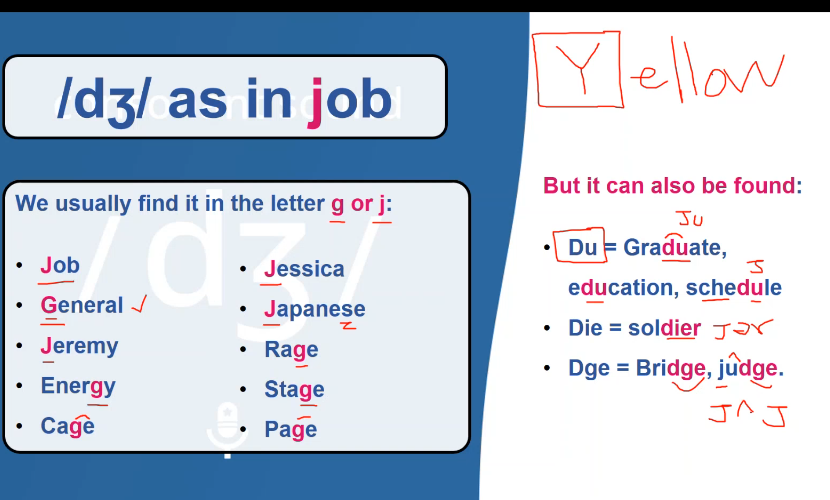
\includegraphics[width=1\textwidth]{images/j_portrait.png}
\end{center}

\href{https://drive.google.com/file/d/1jjBc2nYIz9DPCFFiDWo1M4h6dzX020iO/view?usp=sharing}{Click here to listen}

\begin{longtable}[c]{||l|l||l|l||}
  \hline
  \textcolor{fancyorange}{Word} & \textcolor{fancyorange}{IPA} & \textcolor{fancyorange}{Word} & \textcolor{fancyorange}{IPA} \\
  \hline
  \textbf{\textcolor{fancyorange}{J}ob} & \textipa{/'d\textyogh\textscripta b/} & \textbf{Ima\textcolor{fancyorange}{g}ine} & \textipa{/\textsci'm{\ae}d\textyogh\textsci n/} \\
  \textbf{\textcolor{fancyorange}{Ju}ice} & \textipa{/'d\textyogh us/} & \textbf{Chan\textcolor{fancyorange}{g}e} & \textipa{/'t\textesh e\textsci nd\textyogh/} \\
  \textbf{\textcolor{fancyorange}{J}ump} & \textipa{/'d\textyogh\textturnv mp/} & \textbf{\textcolor{fancyorange}{J}ud\textcolor{fancyorange}{g}e} & \textipa{/'d\textyogh\textturnv d\textyogh/} \\
  \textbf{Ma\textcolor{fancyorange}{g}ic} & \textipa{/'m{\ae}d\textyogh\textsci k/} & \textbf{Apolo\textcolor{fancyorange}{g}ize} & \textipa{/\textschwa'p\textscripta\textlengthmark l\textschwa d\textyogh{\ae}\textsci z/} \\
  \textbf{A\textcolor{fancyorange}{g}e} & \textipa{/'e\textsci d\textyogh/} & \textbf{Char\textcolor{fancyorange}{g}e} & \textipa{/'t\textesh\textscripta\textturnr d\textyogh/} \\
  \textbf{Bud\textcolor{fancyorange}{g}et} & \textipa{/'b\textturnv d\textyogh\textsci t/} & \textbf{\textcolor{fancyorange}{G}eneral} & \textipa{/'d\textyogh en\textschwa r\textschwa l/} \\
  \textbf{Sol\textcolor{fancyorange}{d}ier} & \textipa{/'so\textupsilon ld\textyogh\textschwa\textturnr/} & \textbf{\textcolor{fancyorange}{J}oin} & \textipa{/'d\textyogh\textopeno\textsci n/} \\
  \textbf{Gra\textcolor{fancyorange}{d}uate} & \textipa{/'gr{\ae}d\textyogh ue\textsci t/} & \textbf{En\textcolor{fancyorange}{j}oy} & \textipa{/\textsci n'd\textyogh\textopeno\textsci/} \\
  \textbf{E\textcolor{fancyorange}{d}ucation} & \textipa{/,ed\textyogh\textschwa'ke\textsci\textesh\textschwa n/} & \textbf{Colle\textcolor{fancyorange}{g}e} & \textipa{/'k\textscripta l\textsci d\textyogh/} \\
  \textbf{\textcolor{fancyorange}{J}oke} & \textipa{/'d\textyogh o\textupsilon k/} & \textbf{\textcolor{fancyorange}{D}an\textcolor{fancyorange}{g}erous} & \textipa{/'de\textsci nd\textyogh\textschwa r\textschwa s/} \\
  \textbf{Proce\textcolor{fancyorange}{d}ure} & \textipa{/pr\textschwa'si\textlengthmark d\textyogh\textschwa\textturnr/} & \textbf{Su\textcolor{fancyorange}{gg}estion} & \textipa{/s\textschwa'd\textyogh est\textesh\textschwa n/} \\
  \textbf{Ori\textcolor{fancyorange}{g}inal} & \textipa{/\textschwa'r\textsci d\textyogh\textschwa n\textschwa l/} & \textbf{Sche\textcolor{fancyorange}{d}ule} & \textipa{/'sked\textyogh u\textlengthmark l/} \\
  \hline
\end{longtable}


\begin{enumerate}
  \item I need to get a new \textbf{job}.
  \item Would you like a glass of \textbf{juice}?
  \item Let's add it to our \textbf{budget}.
  \item When are you going to \textbf{graduate}?
  \item I want to get some great \textbf{education}.
  \item You are not following the \textbf{procedure}.
  \item Is that an \textbf{original charger}?
  \item I couldn't \textbf{join} the class on time.
  \item I \textbf{apologize} for the incovenience.
  \item Can I give you a \textbf{suggestion}?
  \item My brother in law used to be a \textbf{soldier} in the army.
  \item Are you happy with yor new \textbf{schedule}?
  \item Honestly, that sounds like a \textbf{dangerous} thing to do.
  \item I'm in \textbf{charge} of handling the company's \textbf{budget}.
  \item You need to enter your \textbf{age} again and save the \textbf{changes}.
\end{enumerate}

\newpage







% ONLY TIPA CODE IS ALLOWED IN THIS FILE
% DO NOT ADD ANYTHING ELSE
\section{Final "-age" sound as in "package", "message" \textipa{\textsci d\textyogh}}
\begin{center}
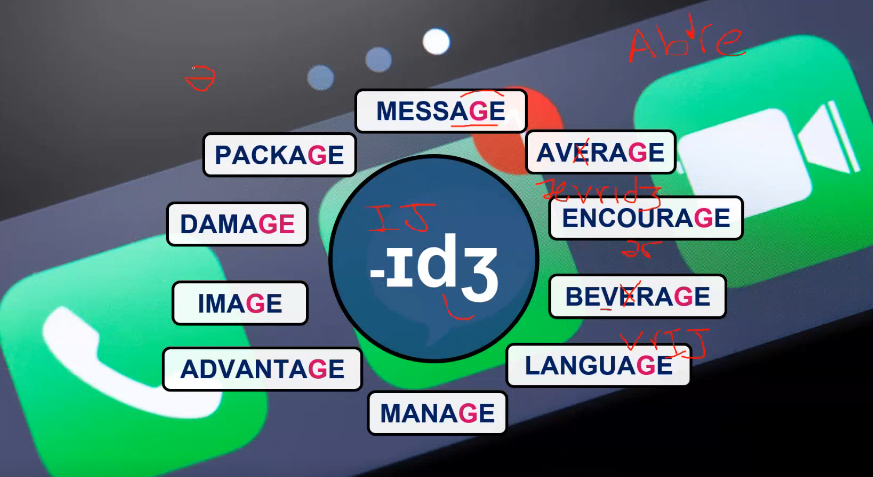
\includegraphics[width=1\textwidth]{images/ihj_portraint.png}
\end{center}

\href{https://drive.google.com/file/d/1rO6usCgIagyJRvrpMbvJ3NY8o-tpPSy-/view?usp=sharing}{Click here to listen}

\begin{longtable}[c]{||l|l||}
  \hline
  \textcolor{fancyorange}{Word} & \textcolor{fancyorange}{IPA} \\
  \hline
  \textbf{Messa\textcolor{fancyorange}{ge}} & \textipa{/'mes\textsci d\textyogh/} \\
  \hline
  \textbf{Packa\textcolor{fancyorange}{ge}} & \textipa{/'p{\ae}k\textsci d\textyogh/} \\
  \hline
  \textbf{Dama\textcolor{fancyorange}{ge}} & \textipa{/'d{\ae}m\textsci d\textyogh/} \\
  \hline
  \textbf{Ima\textcolor{fancyorange}{ge}} & \textipa{/'\textsci m\textsci d\textyogh/} \\
  \hline
  \textbf{Advanta\textcolor{fancyorange}{ge}} & \textipa{/\textschwa d'v{\ae}nt\textsci d\textyogh/} \\
  \hline
  \textbf{Mana\textcolor{fancyorange}{ge}} & \textipa{/'m{\ae}n\textsci d\textyogh/} \\
  \hline
  \textbf{Langua\textcolor{fancyorange}{ge}} & \textipa{/'l{\ae}\ng gw\textsci d\textyogh/} \\
  \hline
  \textbf{Bevera\textcolor{fancyorange}{ge}} & \textipa{/'bev\textschwa r\textsci d\textyogh/} \\
  \hline
  \textbf{Encoura\textcolor{fancyorange}{ge}} & \textipa{/\textsci n'k\textschwa\textlengthmark\textturnr\textsci d\textyogh/} \\
  \hline
  \textbf{Avera\textcolor{fancyorange}{ge}} & \textipa{/'{\ae}v\textschwa r\textsci d\textyogh/} \\
  \hline  
\end{longtable}


\begin{enumerate}
  \item I got a \textbf{message} saying that I won a pickup truck. Should I believe it?
  \item Did you receive the \textbf{package} I sent you last week? It said it was delivered.
  \item I can't believe you \textbf{damaged} my car. Are you going to pay for it?
  \item Do you think celebrities need to have a good public \textbf{image}? Why?
  \item What are some of the \textbf{advantages} of studying from home? Do you think you would prefer to study in person?
  \item How do you \textbf{manage} to study for 8 hours every day?
  \item As Spanish speakers, do you think we should also work on how we use our \textbf{language}?
  \item What kind of \textbf{beverage} do you usually have with your breakfast or lunch?
  \item How can I \textbf{encourage} someone to practice their English? Any advice?
  \item On \textbf{average}, how many hours do you sleep every night?
\end{enumerate}

\newpage







% ONLY TIPA CODE IS ALLOWED IN THIS FILE
% DO NOT ADD ANYTHING ELSE
\section{"V" sound as in "very" \textipa{/v/}}
\begin{center}
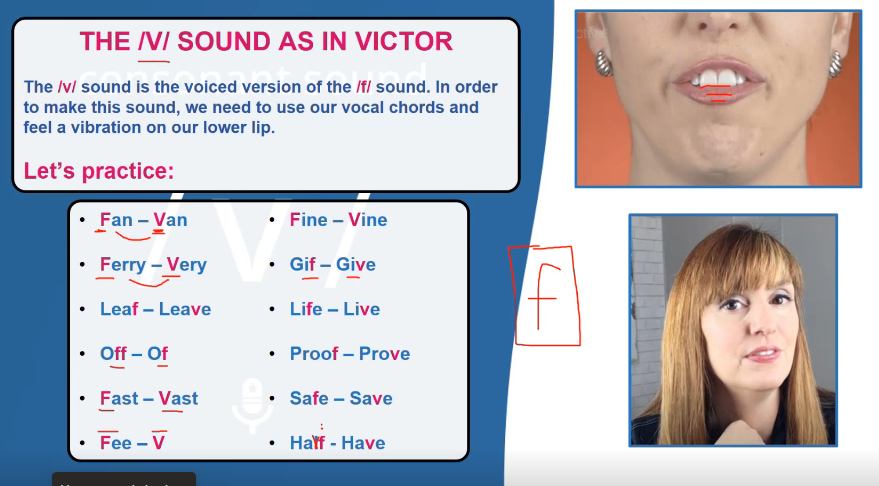
\includegraphics[width=1\textwidth]{images/v_portrait.png}
\end{center}

\href{https://drive.google.com/file/d/1C9-dVurAhFHisFtu7BXRSUUTWpi2ZDxw/view?usp=sharing}{Click here to listen}

\begin{longtable}[c]{||l|l||l|l||}
  \hline
  \textcolor{fancyorange}{Word} & \textcolor{fancyorange}{IPA} & \textcolor{fancyorange}{Word} & \textcolor{fancyorange}{IPA} \\
  \hline
  \textbf{\textcolor{fancyorange}{V}ery} & \textipa{/'veri/} & \textbf{Ri\textcolor{fancyorange}{v}er} & \textipa{/'r\textsci v\textschwa\textturnr/} \\
  \hline
  \textbf{Ha\textcolor{fancyorange}{v}e} & \textipa{/'h{\ae}v/} & \textbf{Ser\textcolor{fancyorange}{v}ice} & \textipa{/'s\textschwa\textlengthmark\textturnr v\textsci s/} \\
  \hline
  \textbf{Lea\textcolor{fancyorange}{v}e} & \textipa{/'li\textlengthmark v/} & \textbf{\textcolor{fancyorange}{V}olume} & \textipa{/'v\textscripta\textlengthmark lju\textlengthmark m/} \\
  \hline
  \textbf{Sa\textcolor{fancyorange}{v}e} & \textipa{/'se\textsci v/} & \textbf{Se\textcolor{fancyorange}{v}en} & \textipa{/'sev\textschwa n/} \\
  \hline
  \textbf{\textcolor{fancyorange}{V}acation} & \textipa{/,ve\textsci'ke\textsci\textesh\textschwa n/} & \textbf{Tra\textcolor{fancyorange}{v}el} & \textipa{/'tr{\ae}v\textschwa l/} \\
  \hline
  \textbf{\textcolor{fancyorange}{V}ariety} & \textipa{/v\textschwa'r{\ae}\textsci\textschwa ti/} & \textbf{Beha\textcolor{fancyorange}{v}e} & \textipa{/b\textsci'he\textsci v/} \\
  \hline
  \textbf{\textcolor{fancyorange}{V}egan} & \textipa{/'vi\textlengthmark g\textschwa n/} & \textbf{Bra\textcolor{fancyorange}{v}e} & \textipa{/'bre\textsci v/} \\
  \hline
  \textbf{\textcolor{fancyorange}{V}erb} & \textipa{/'v\textschwa\textlengthmark\textturnr b/} & \textbf{Dri\textcolor{fancyorange}{v}e} & \textipa{/'dr{\ae}\textsci v/} \\
  \hline
  \textbf{\textcolor{fancyorange}{V}iew} & \textipa{/'vju\textlengthmark/} & \textbf{Gi\textcolor{fancyorange}{v}e} & \textipa{/'g\textsci v/} \\
  \hline
  \textbf{\textcolor{fancyorange}{V}oice} & \textipa{/'v\textopeno\textsci s/} & \textbf{Lo\textcolor{fancyorange}{v}e} & \textipa{/'l\textturnv v/} \\
  \hline
  \textbf{\textcolor{fancyorange}{V}ote} & \textipa{/'vo\textupsilon t/} & \textbf{Mo\textcolor{fancyorange}{v}e} & \textipa{/'mu\textlengthmark v/} \\
  \hline
  \textbf{Co\textcolor{fancyorange}{v}er} & \textipa{/'k\textturnv v\textschwa\textturnr/} & \textbf{O\textcolor{fancyorange}{f}} & \textipa{/'A\textlengthmark v/} \\
  \hline
  \textbf{E\textcolor{fancyorange}{v}en} & \textipa{/'i\textlengthmark v\textschwa n/} & \textbf{Pro\textcolor{fancyorange}{v}e} & \textipa{/'pru\textlengthmark v/} \\
  \hline
  \textbf{E\textcolor{fancyorange}{v}ent} & \textipa{/\textsci'vent/} & \textbf{Ser\textcolor{fancyorange}{v}e} & \textipa{/'s\textschwa\textlengthmark\textturnr v/} \\
  \hline
  \textbf{E\textcolor{fancyorange}{v}er} & \textipa{/'ev\textschwa\textturnr/} & \textbf{Slee\textcolor{fancyorange}{v}e} & \textipa{/'sli\textlengthmark v/} \\
  \hline
  \textbf{Fa\textcolor{fancyorange}{v}or} & \textipa{/'fe\textsci v\textschwa\textturnr/} & \textbf{Sol\textcolor{fancyorange}{v}e} & \textipa{/'s\textscripta\textlengthmark lv/} \\
  \hline
  \textbf{In\textcolor{fancyorange}{v}ite} & \textipa{/\textsci n'v{\ae}\textsci t/} & \textbf{Sto\textcolor{fancyorange}{v}e} & \textipa{/'sto\textupsilon v/} \\
  \hline
  \textbf{Le\textcolor{fancyorange}{v}el} & \textipa{/'lev\textschwa l/} & \textbf{Wa\textcolor{fancyorange}{v}e} & \textipa{/'we\textsci v/} \\
  \hline
  \textbf{Mo\textcolor{fancyorange}{v}ie} & \textipa{/'mu\textlengthmark vi/} & \textbf{O\textcolor{fancyorange}{v}en} & \textipa{/'\textturnv v\textschwa n/} \\
  \hline
  \textbf{Ne\textcolor{fancyorange}{v}er} & \textipa{/'nev\textschwa\textturnr/} & \textbf{Inter\textcolor{fancyorange}{v}iew} & \textipa{/'\textsci nt\textschwa\textturnr vju\textlengthmark/} \\
  \hline
  \textbf{O\textcolor{fancyorange}{v}er} & \textipa{/'o\textupsilon v\textschwa\textturnr/} & \textbf{\textcolor{fancyorange}{V}isit} & \textipa{/'v\textsci z\textsci t/} \\
  \hline
  \textbf{Pri\textcolor{fancyorange}{v}ate} & \textipa{/'pr{\ae}\textsci v\textschwa t/} &  & \\
  \hline
\end{longtable}




\begin{enumerate}
  \item I'm \textbf{very} excited about my graduation.
  \item Take the box and \textbf{leave} it outside.
  \item Your customer \textbf{service} is excellent.
  \item Are you ready for your next \textbf{interview}?
  \item \textbf{Move} out of the way!
  \item Could you just turn down the \textbf{volume}?
  \item I \textbf{have never} seen someone so \textbf{brave}.
  \item \textbf{Even} if I don't go to the \textbf{event}, I'll \textbf{give} you a present.
  \item Could you do me a \textbf{favor}?
  \item We had a \textbf{variety} of \textbf{activities} on our \textbf{vacation}.
  \item I \textbf{love driving} around with my music on.
  \item I lost my \textbf{voice} after taking calls for a day.
  \item Are you \textbf{even} paying attention to me?
  \item \textbf{Save} the changes and let's go watch a movie.
  \item Why didn't you \textbf{invite} me to your special \textbf{event}?
  \item \textbf{I've never travelled} to another country.
\end{enumerate}

\newpage








% annexes
\chapter{Annexes}
\section{}

\begin{tabular}{||l|l|p{3.5cm}||}
    \hline
    \textbf{Sound} & \textbf{IPA Symbol} & \textbf{TIPA command (for \textbackslash textipa\{\})} \\
    \hline\hline
  
    \multicolumn{3}{||c||}{\textbf{Consonants}} \\
    \hline
    Voiceless bilabial plosive & \textipa{p} & \texttt{p} \\
    Voiced bilabial plosive & \textipa{b} & \texttt{b} \\
    Voiceless alveolar plosive & \textipa{t} & \texttt{t} \\
    Voiced alveolar plosive & \textipa{d} & \texttt{d} \\
    Voiceless velar plosive & \textipa{k} & \texttt{k} \\
    Voiced velar plosive & \textipa{g} & \texttt{g} \\
    Bilabial nasal & \textipa{m} & \texttt{m} \\
    Alveolar nasal & \textipa{n} & \texttt{n} \\
    Velar nasal & \textipa{\ng} & \texttt{ng} \\
    Voiceless labiodental fricative & \textipa{f} & \texttt{f} \\
    Voiced labiodental fricative & \textipa{v} & \texttt{v} \\
    Voiceless dental fricative & \textipa{\texttheta} & \texttt{texttheta} \\
    Voiced dental fricative & \textipa{\dh} & \texttt{dh} \\
    Voiceless alveolar fricative & \textipa{s} & \texttt{s} \\
    Voiced alveolar fricative & \textipa{z} & \texttt{z} \\
    Voiceless postalveolar fricative & \textipa{\textesh} & \texttt{textesh} \\
    Voiced postalveolar fricative & \textipa{\textyogh} & \texttt{textyogh} \\
    Voiceless glottal fricative & \textipa{h} & \texttt{h} \\
    Voiceless postalveolar affricate & \textipa{t\textesh} & \texttt{ttextesh} \\
    Voiced postalveolar affricate & \textipa{d\textyogh} & \texttt{dtextyogh} \\
    Alveolar approximant & \textipa{\textturnr} & \texttt{textturnr} \\
    Palatal approximant & \textipa{j} & \texttt{j} \\
    Labio-velar approximant & \textipa{w} & \texttt{w} \\
    Alveolar lateral approximant & \textipa{l} & \texttt{l} \\
    \hline
  
    \multicolumn{3}{||c||}{\textbf{Vowels}} \\
    \hline
    Close front unrounded vowel & \textipa{i} & \texttt{i} \\
    Near-close near-front unrounded vowel & \textipa{\textsci} & \texttt{textsci} \\
    Close-mid front unrounded vowel & \textipa{e} & \texttt{e} \\
    Open-mid front unrounded vowel & \textipa{\textepsilon} & \texttt{textepsilon} \\
    Near-open front unrounded vowel & \textipa{{\ae}} & \texttt{{\ae}} \\
    Mid central vowel (schwa) & \textipa{\textschwa} & \texttt{textschwa} \\
    Open-mid back unrounded vowel & \textipa{\textturnv} & \texttt{textturnv} \\
    Near-close near-back rounded vowel & \textipa{\textupsilon} & \texttt{textupsilon} \\
    Close back rounded vowel & \textipa{u} & \texttt{u} \\
    Open back unrounded vowel & \textipa{\textscripta} & \texttt{textscripta} \\
    Open-mid back rounded vowel & \textipa{\textopeno} & \texttt{textopeno} \\
    \hline
  
    \multicolumn{3}{||c||}{\textbf{Diphthongs (as combinations)}} \\
    \hline
    \textipa{/e\textsci/} (as in face) & \textipa{e\textsci} & \texttt{e textsci} \\
    \textipa{/{\ae}\textsci/} (as in price) & \textipa{{\ae}\textsci} & \texttt{{\ae} textsci} \\
    \textipa{/\textopeno\textsci/} (as in choice) & \textipa{\textopeno\textsci} & \texttt{textopeno textsci} \\
    \textipa{/{\ae}\textupsilon/} (as in mouth) & \textipa{{\ae}\textupsilon} & \texttt{{\ae} textupsilon} \\
    \textipa{/o\textupsilon/} (as in goat) & \textipa{o\textupsilon} & \texttt{o textupsilon} \\
    \hline  
  \end{tabular}

\end{document}

